\documentclass{article}
\usepackage[UTF8]{ctex}
% Replace `letterpaper' with`a4paper' for UK/EU standard size
\usepackage[a4paper,top=2cm,bottom=2cm,left=3cm,right=3cm,marginparwidth=1.75cm]{geometry}

% Useful packages
\usepackage{amsmath}
\usepackage{mathrsfs,amsmath}
\usepackage{graphicx}
\usepackage[colorlinks=true, allcolors=blue]{hyperref}
\usepackage{graphicx} %插入图片的宏包
\usepackage{float} %设置图片浮动位置的宏包
\usepackage{subfigure} %插入多图时用子图显示的宏包
\usepackage{parskip}
\usepackage{indentfirst} 
\setlength{\parindent}{2em}
\usepackage{hyperref}  
\usepackage{tikz}
\allowdisplaybreaks
\usepackage{multirow}
\usepackage{amsmath}
\usepackage{amsfonts,amssymb} 
\usepackage{xcolor} % 用于显示颜色
\usepackage{listings} % 用于插入代码
\lstset{
	basicstyle          =   \sffamily,          % 基本代码风格
	keywordstyle        =   \bfseries,          % 关键字风格
	commentstyle        =   \rmfamily\itshape,  % 注释的风格,斜体
	stringstyle         =   \ttfamily,  % 字符串风格
	flexiblecolumns,                % 别问为什么,加上这个
	numbers             =   left,   % 行号的位置在左边
	showspaces          =   false,  % 是否显示空格,显示了有点乱,所以不现实了
	numberstyle         =   \zihao{-5}\ttfamily,    % 行号的样式,小五号,tt等宽字体
	showstringspaces    =   false,
	captionpos          =   t,      % 这段代码的名字所呈现的位置,t指的是top上面
	frame               =   lrtb,   % 显示边框
}

\lstdefinestyle{Python}{
	language        =   Python, % 语言选Python
	basicstyle      =   \zihao{-5}\ttfamily,
	numberstyle     =   \zihao{-5}\ttfamily,
	keywordstyle    =   \color{blue},
	keywordstyle    =   [2] \color{teal},
	stringstyle     =   \color{magenta},
	commentstyle    =   \color{red}\ttfamily,
	breaklines      =   true,   % 自动换行,建议不要写太长的行
	columns         =   fixed,  % 如果不加这一句,字间距就不固定,很丑,必须加
	basewidth       =   0.5em,
}

\title{图像处理与可视化 Homework4 报告}
\author{林子开 21307110161}
\begin{document}
	\maketitle
	\tableofcontents

\section{频率域滤波}

\subsection{平滑}

\subsubsection{频域滤波器:高斯低通滤波器(GLPF)}
使用的高斯低通滤波器如下

\[
H(u,v) = \exp[-D^2(u,v)/2\sigma^2]	
\]
其中
\[
D^2(u,v) = (u-u_0)^2 + (v-v_0)^2	
\]
$(u_0,v_0)$ 表示频域的中心点,$\sigma$表示高斯滤波器的标准差,$\sigma$越大,滤波后的频域图像会
保留越多高频信号。

\subsubsection{Python代码实现}
Python代码实现频域低通滤波的代码如下,
其中,\textbf{频域滤波的五个标准步骤:}
\begin{enumerate}
	\item 填充
	\item 中心化,DFT
	\item 频域滤波
	\item IDFT,去中心化
	\item 提取左上象限图像
\end{enumerate}
\textbf{均已写在smooth函数中的注释中},敬请读者结合Python代码审阅。

\lstinputlisting[style = Python,
caption={Python codes for smoothing by GLPF},
label = {GLPF}]{1_1_smoothing_GLPF.py}

\subsubsection{效果展示}

以下展示了原图的频谱、滤波后的频谱以及滤波后的效果。

% \paragraph{原图以及原图频谱}
\begin{figure}[H]
    \centering
    \subfigure[原图]
    {\label{ori.sub.1} 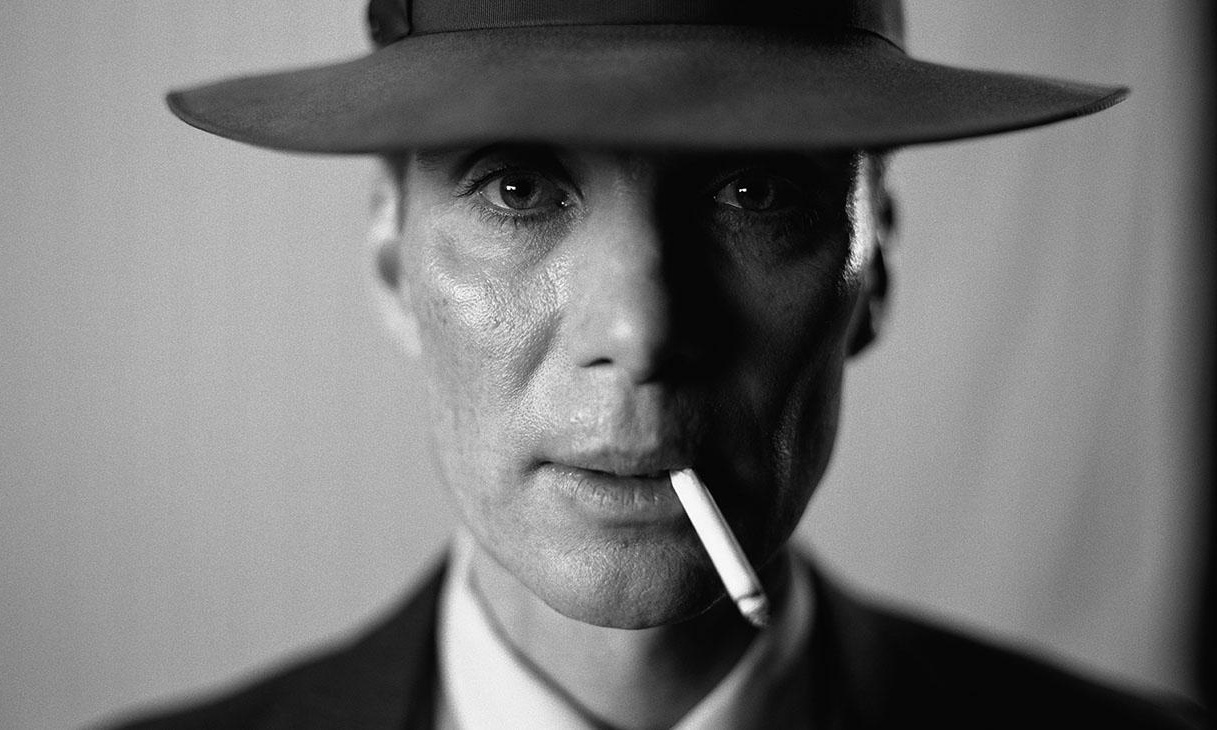
\includegraphics[width=0.47\textwidth]{test.jpeg}}
    \,    
    \subfigure[原图频谱(取对数)]
    {\label{ori.sub.2} 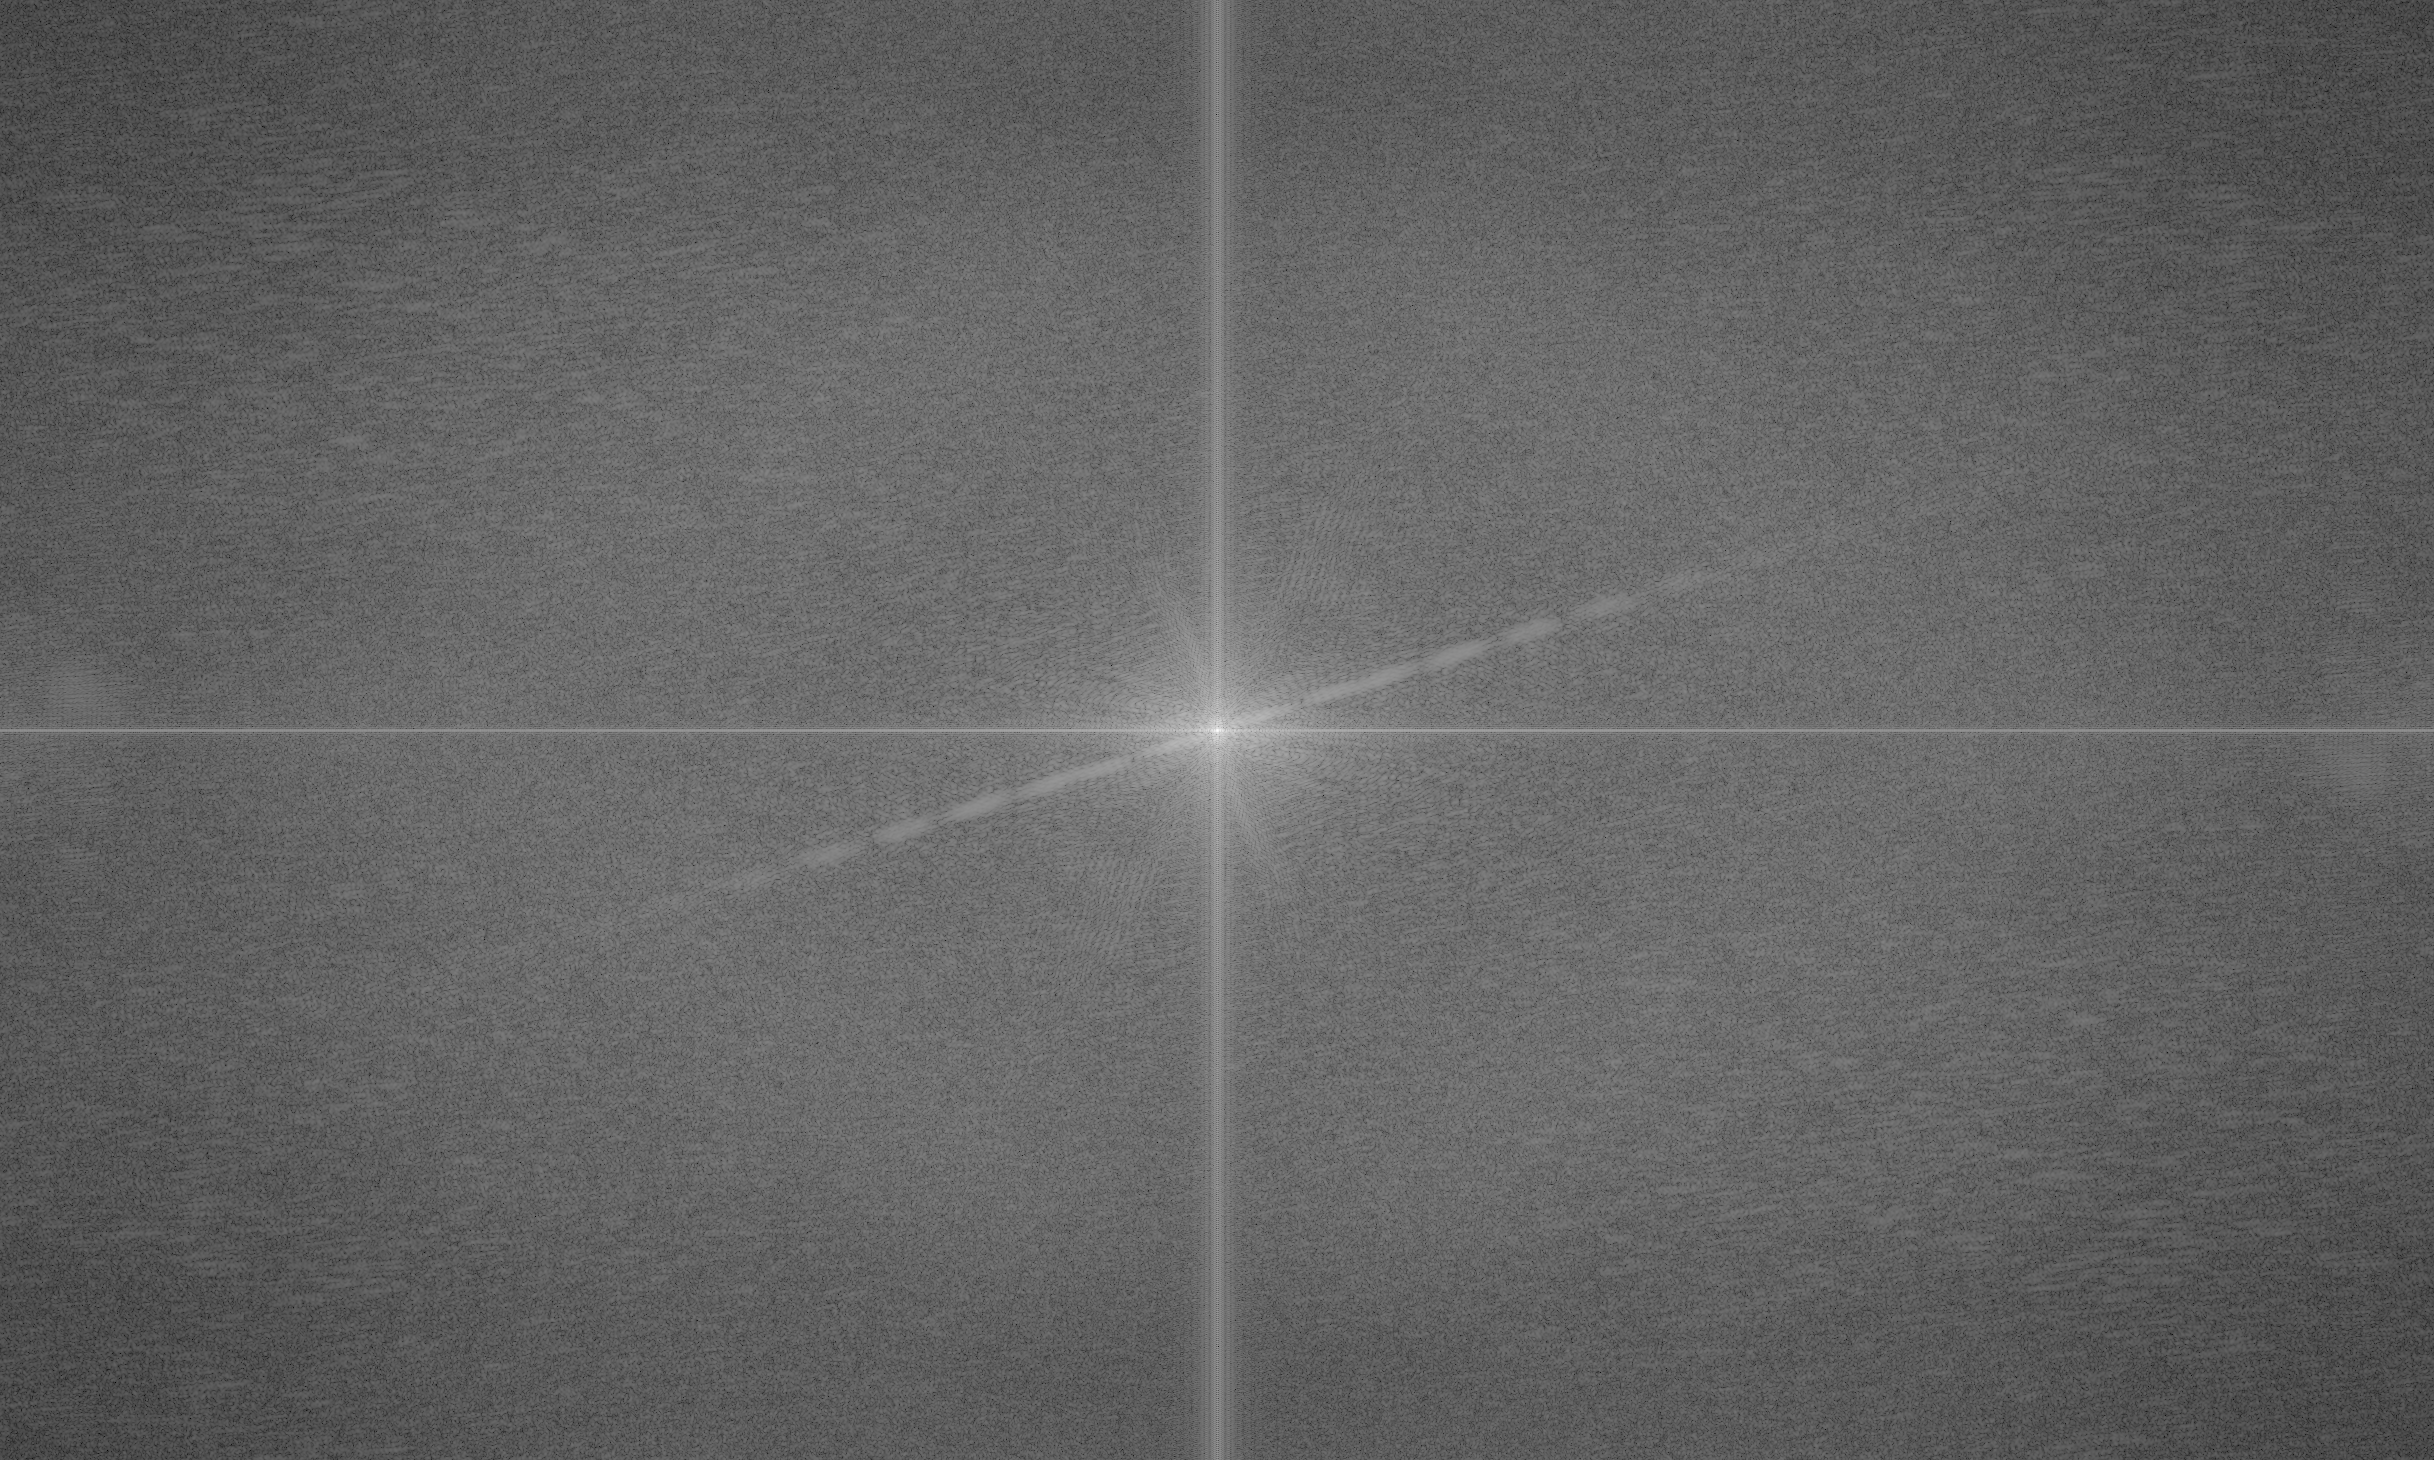
\includegraphics[width=0.47\textwidth]{smooth_result_Gauss//sigma=10 frequency.png}}
    \caption{原图与原图频谱}\label{ori.main} 
\end{figure}

% \paragraph{$\sigma=20$的频域滤波结果与效果图}
\begin{figure}[H]
    \centering
    \subfigure[频域滤波结果(取对数)]
    {\label{} 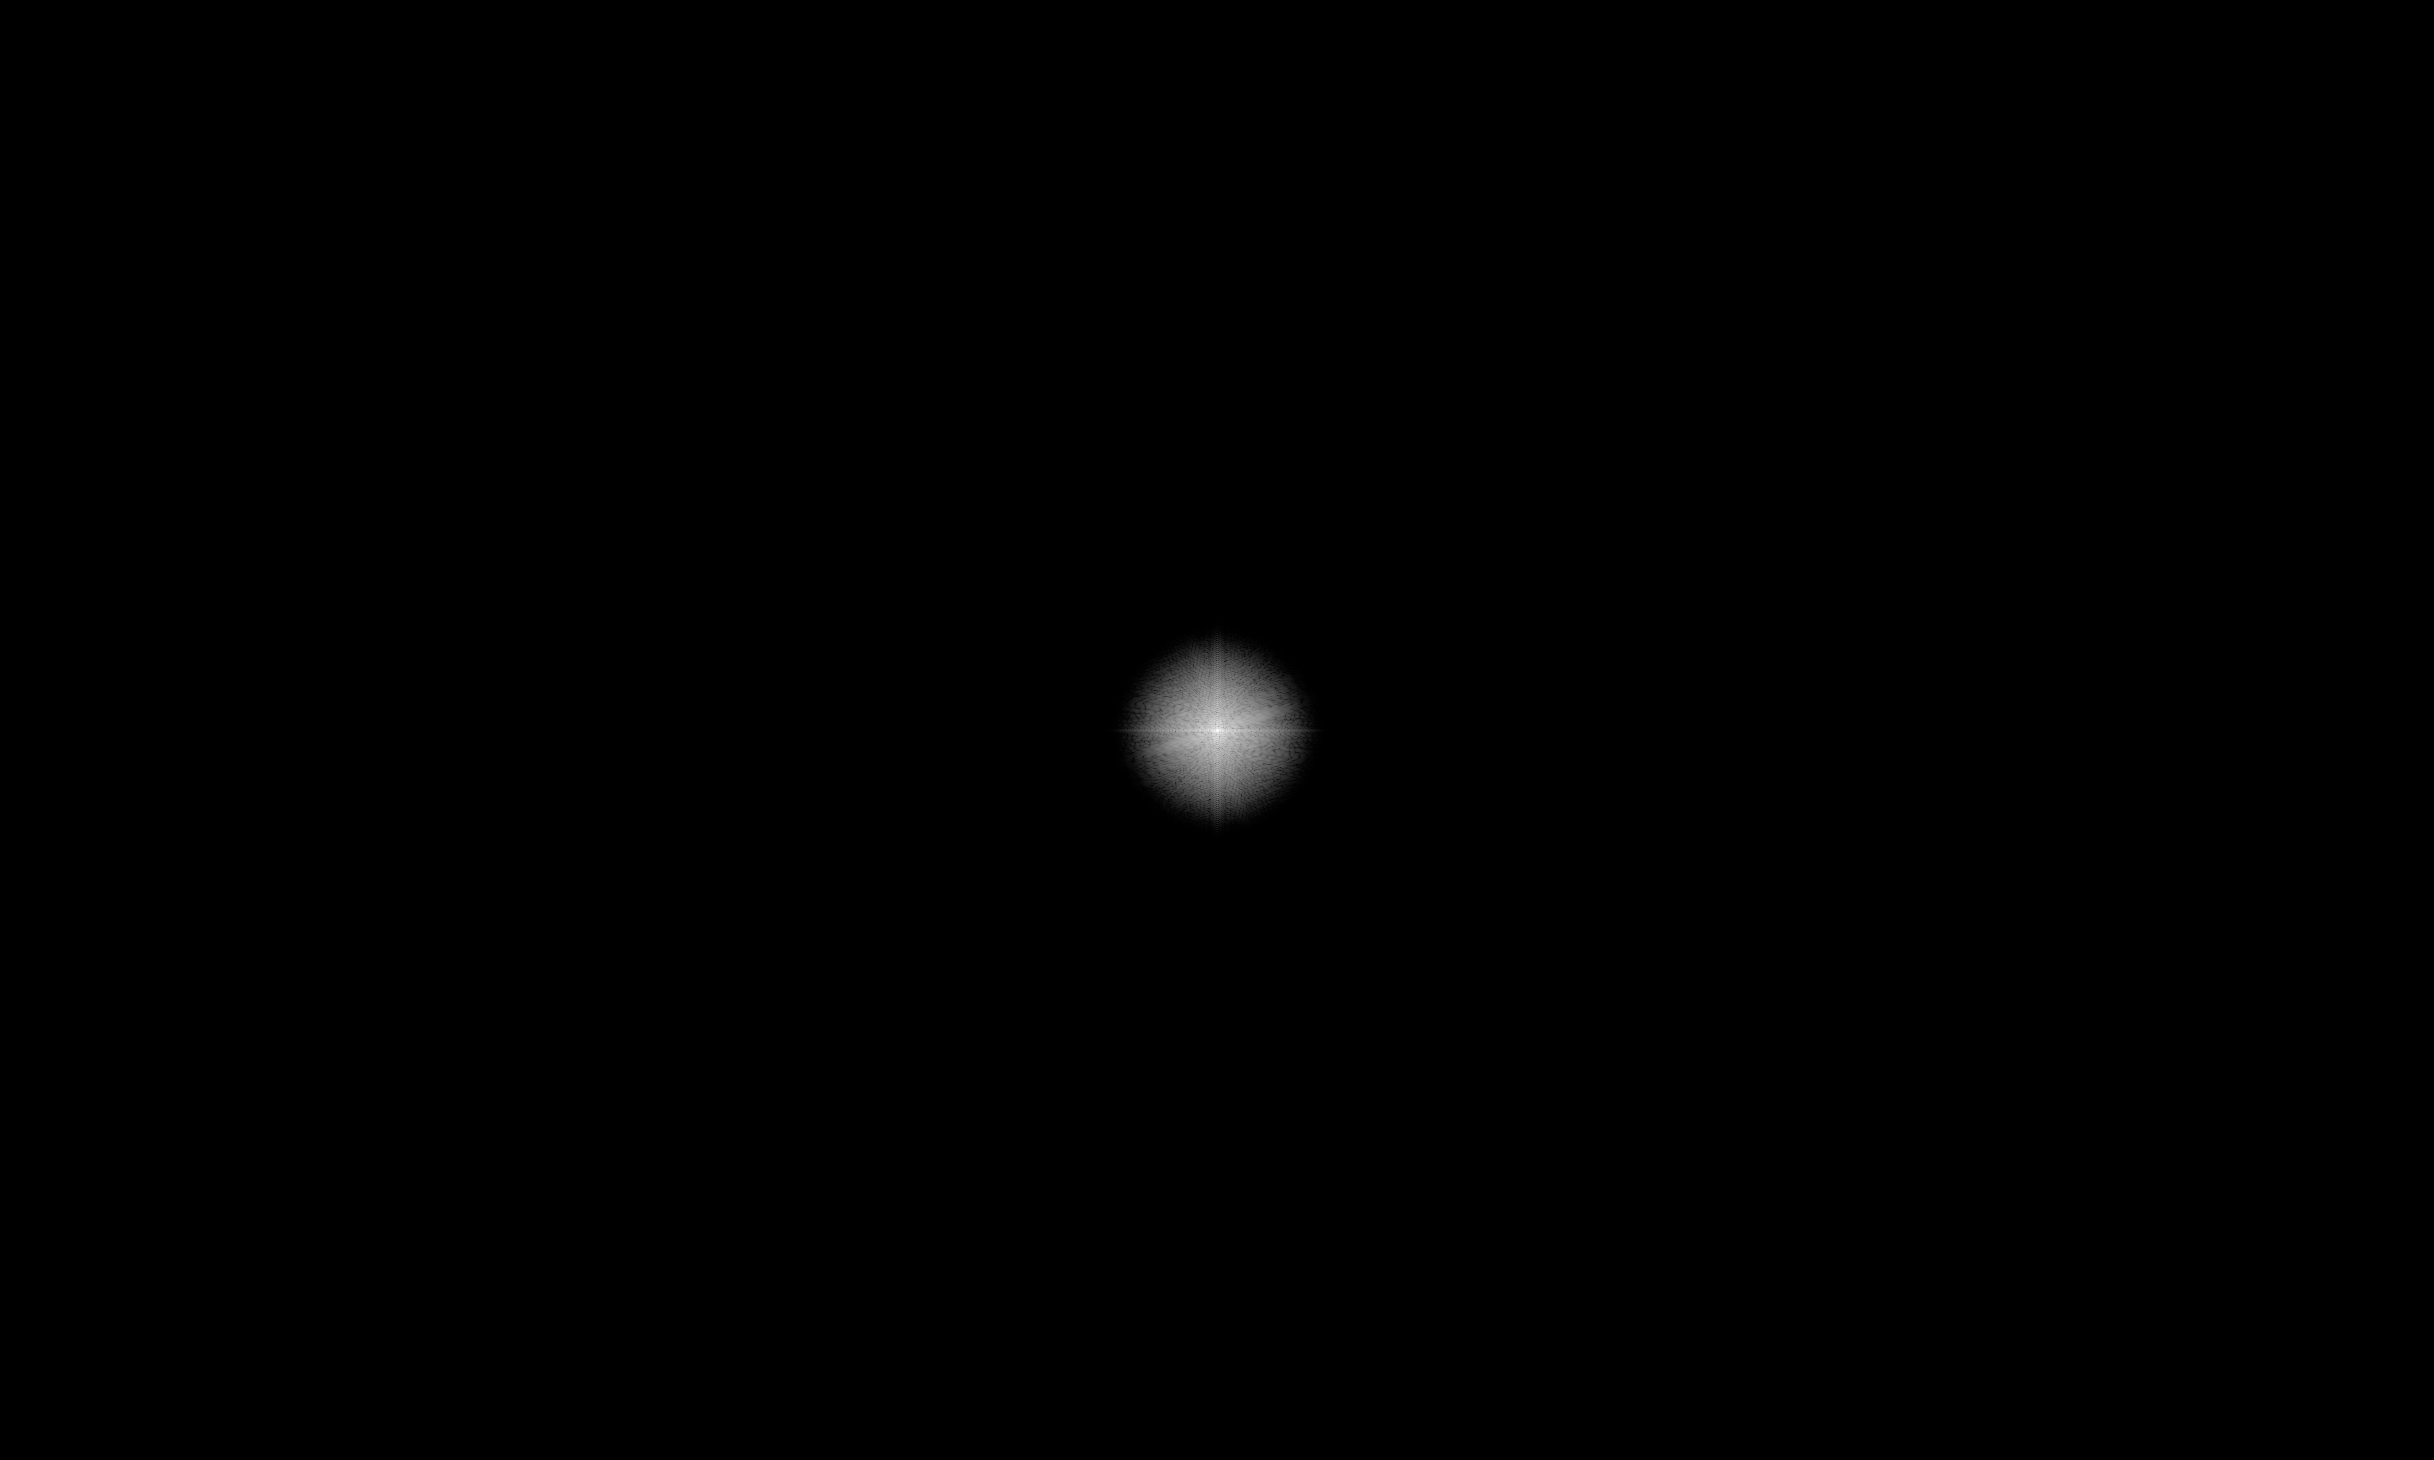
\includegraphics[width=0.47\textwidth]{smooth_result_Gauss//sigma=20 filtered frequency.png}}
    \,    
    \subfigure[滤波效果]
    {\label{} 
\includegraphics[width=0.47\textwidth]{smooth_result_Gauss//sigma=20 filtered figure.png}}
    \caption{$\sigma=20$的频域滤波结果与效果图}\label{} 
\end{figure}


% \paragraph{$\sigma=40$的频域低通滤波结果与效果图}
\begin{figure}[H]
    \centering
    \subfigure[频域低通滤波结果(取对数)]
    {\label{} 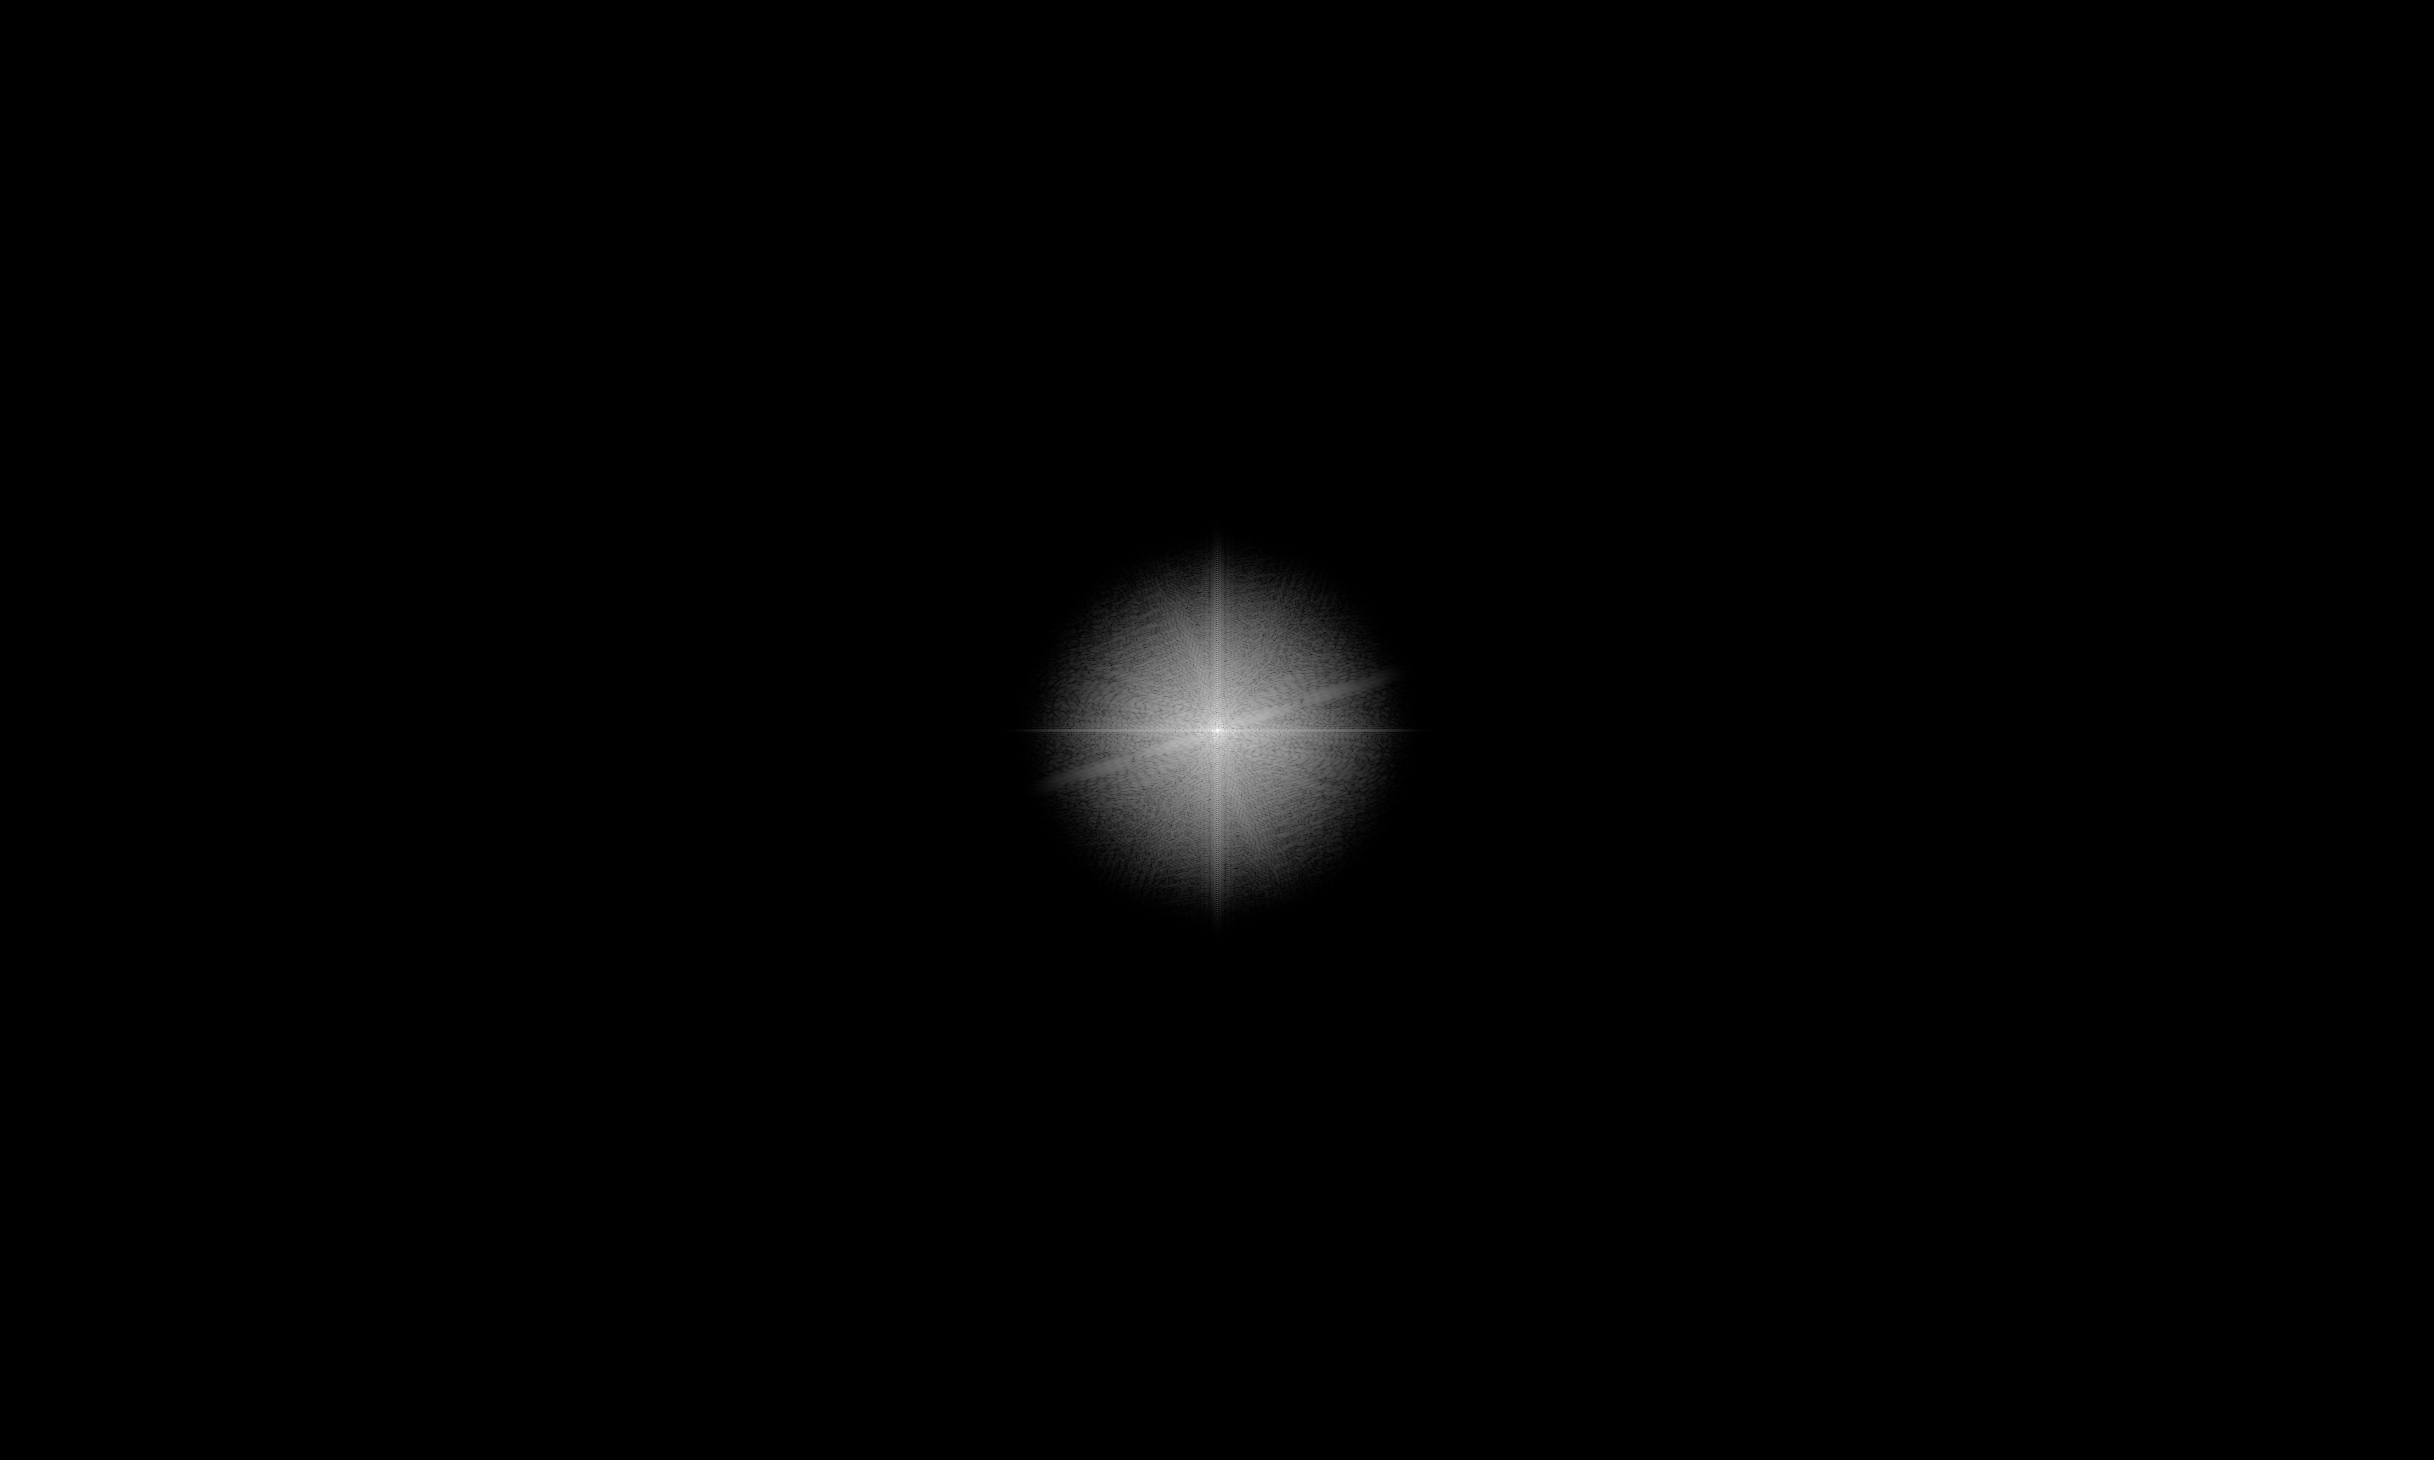
\includegraphics[width=0.47\textwidth]{smooth_result_Gauss//sigma=40 filtered frequency.png}}
    \,    
    \subfigure[滤波效果]
    {\label{} 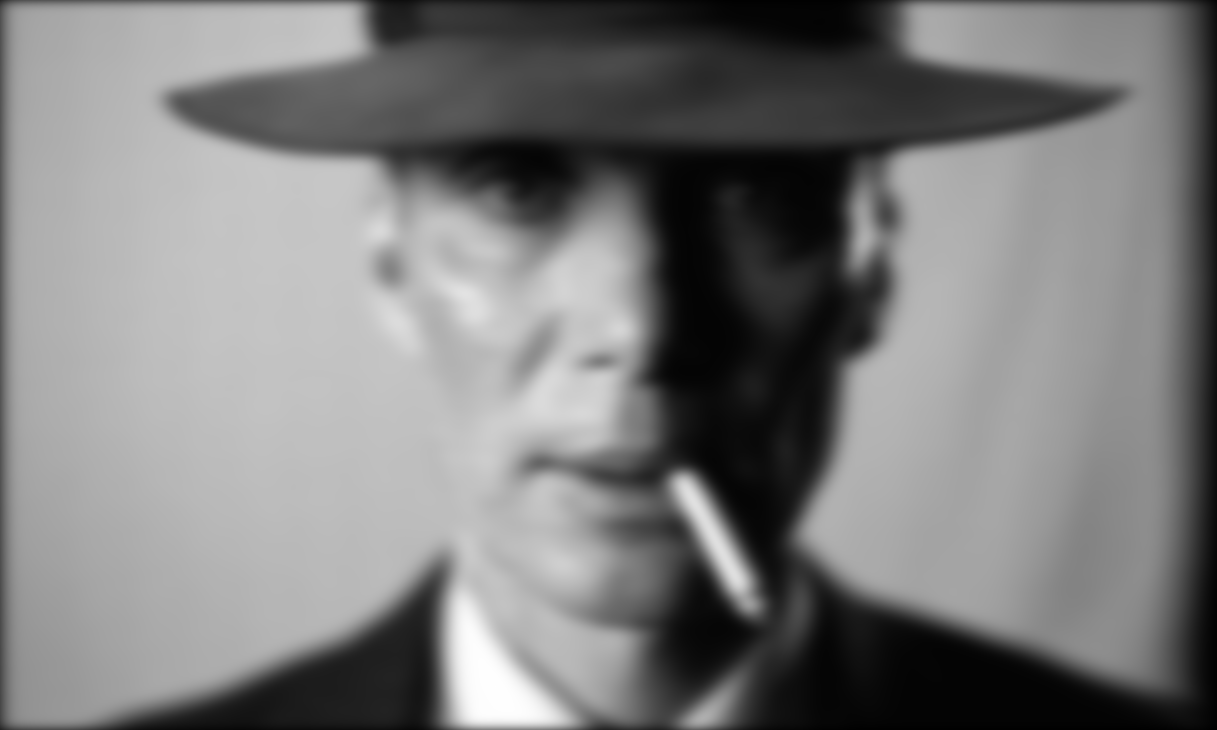
\includegraphics[width=0.47\textwidth]{smooth_result_Gauss//sigma=40 filtered figure.png}}
    \caption{$\sigma=40$的频域低通滤波结果与效果图}\label{} 
\end{figure}

% \paragraph{$\sigma=60$的频域低通滤波结果与效果图}
\begin{figure}[H]
    \centering
    \subfigure[频域低通滤波结果(取对数)]
    {\label{} 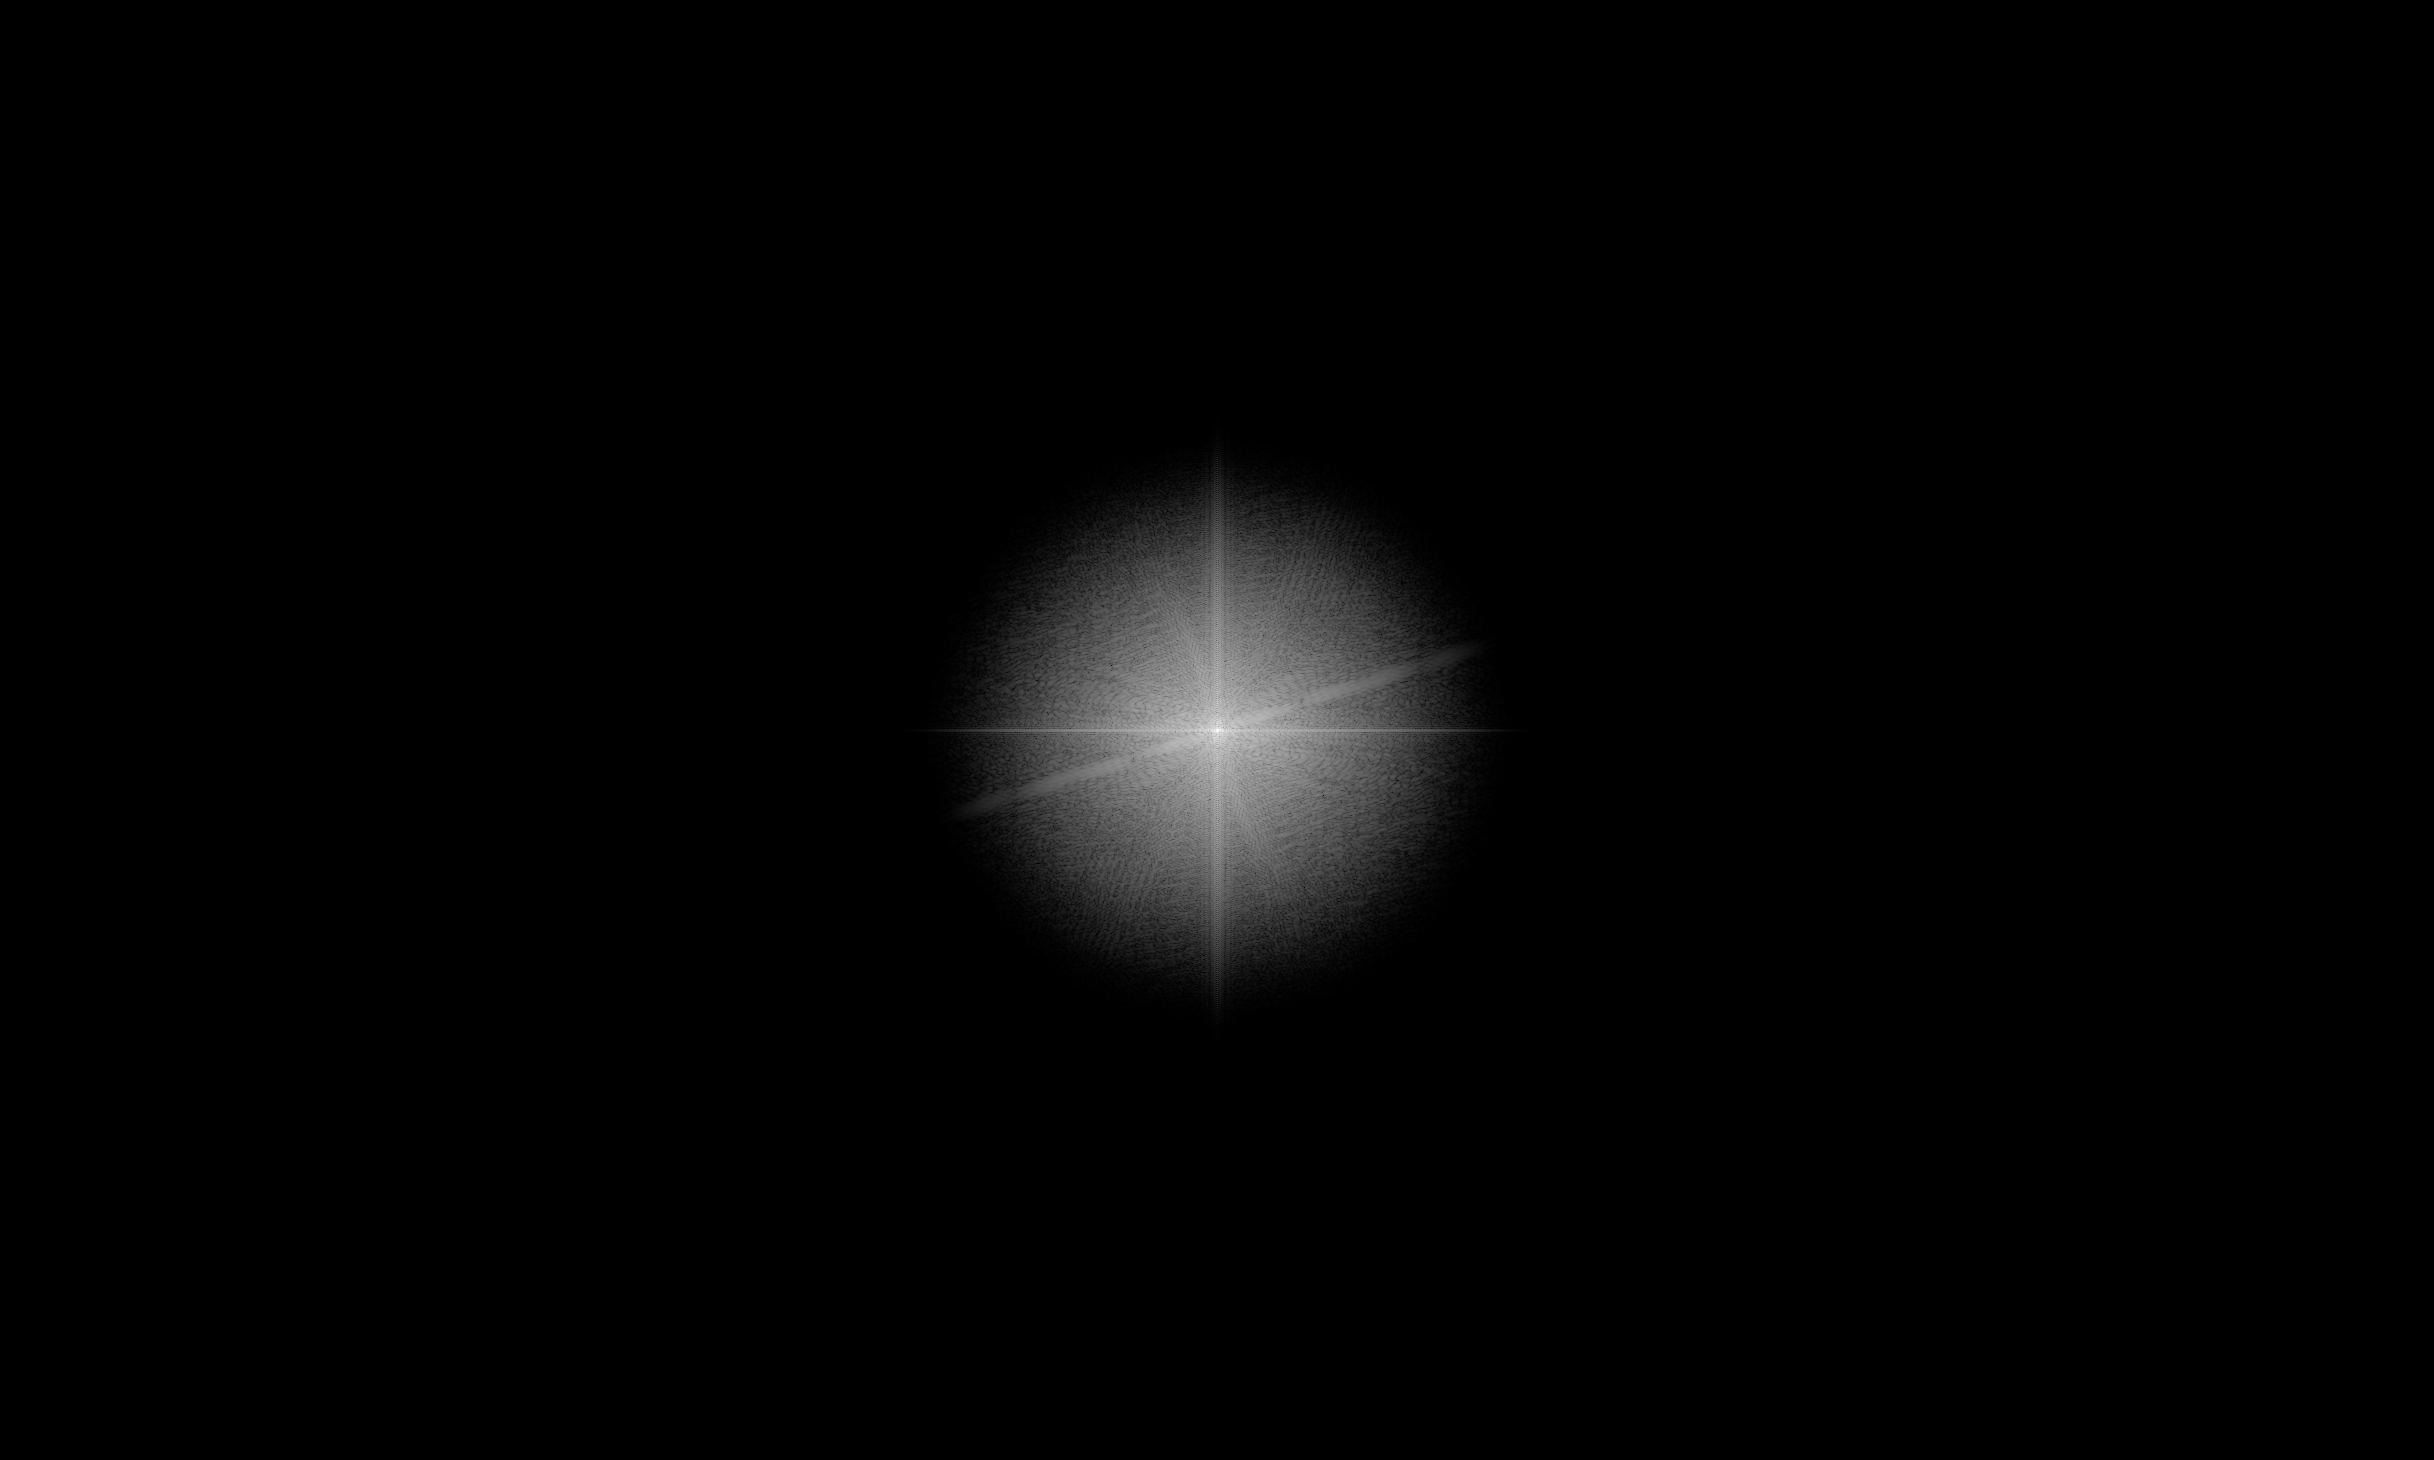
\includegraphics[width=0.47\textwidth]{smooth_result_Gauss//sigma=60 filtered frequency.png}}
    \,    
    \subfigure[滤波效果]
    {\label{} 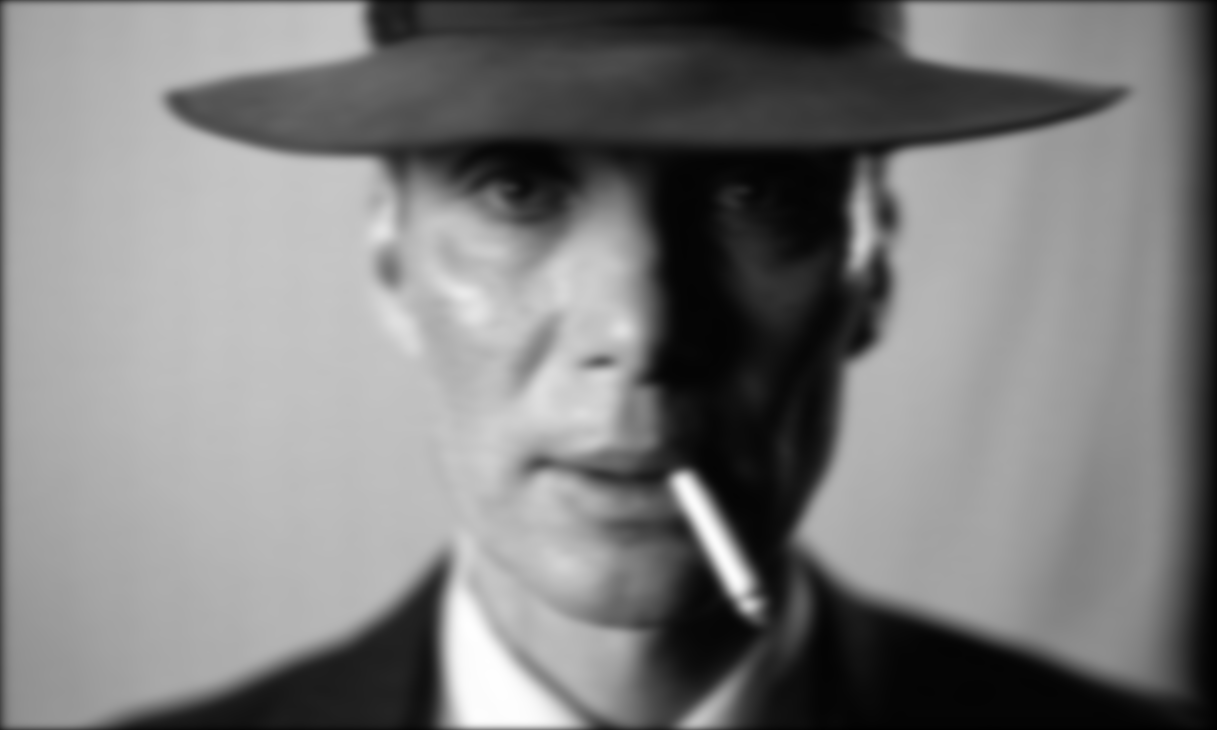
\includegraphics[width=0.47\textwidth]{smooth_result_Gauss//sigma=60 filtered figure.png}}
    \caption{$\sigma=60$的频域低通滤波结果与效果图}\label{} 
\end{figure}


% \paragraph{$\sigma=80$的频域低通滤波结果与效果图}
\begin{figure}[H]
    \centering
    \subfigure[频域低通滤波结果(取对数)]
    {\label{} 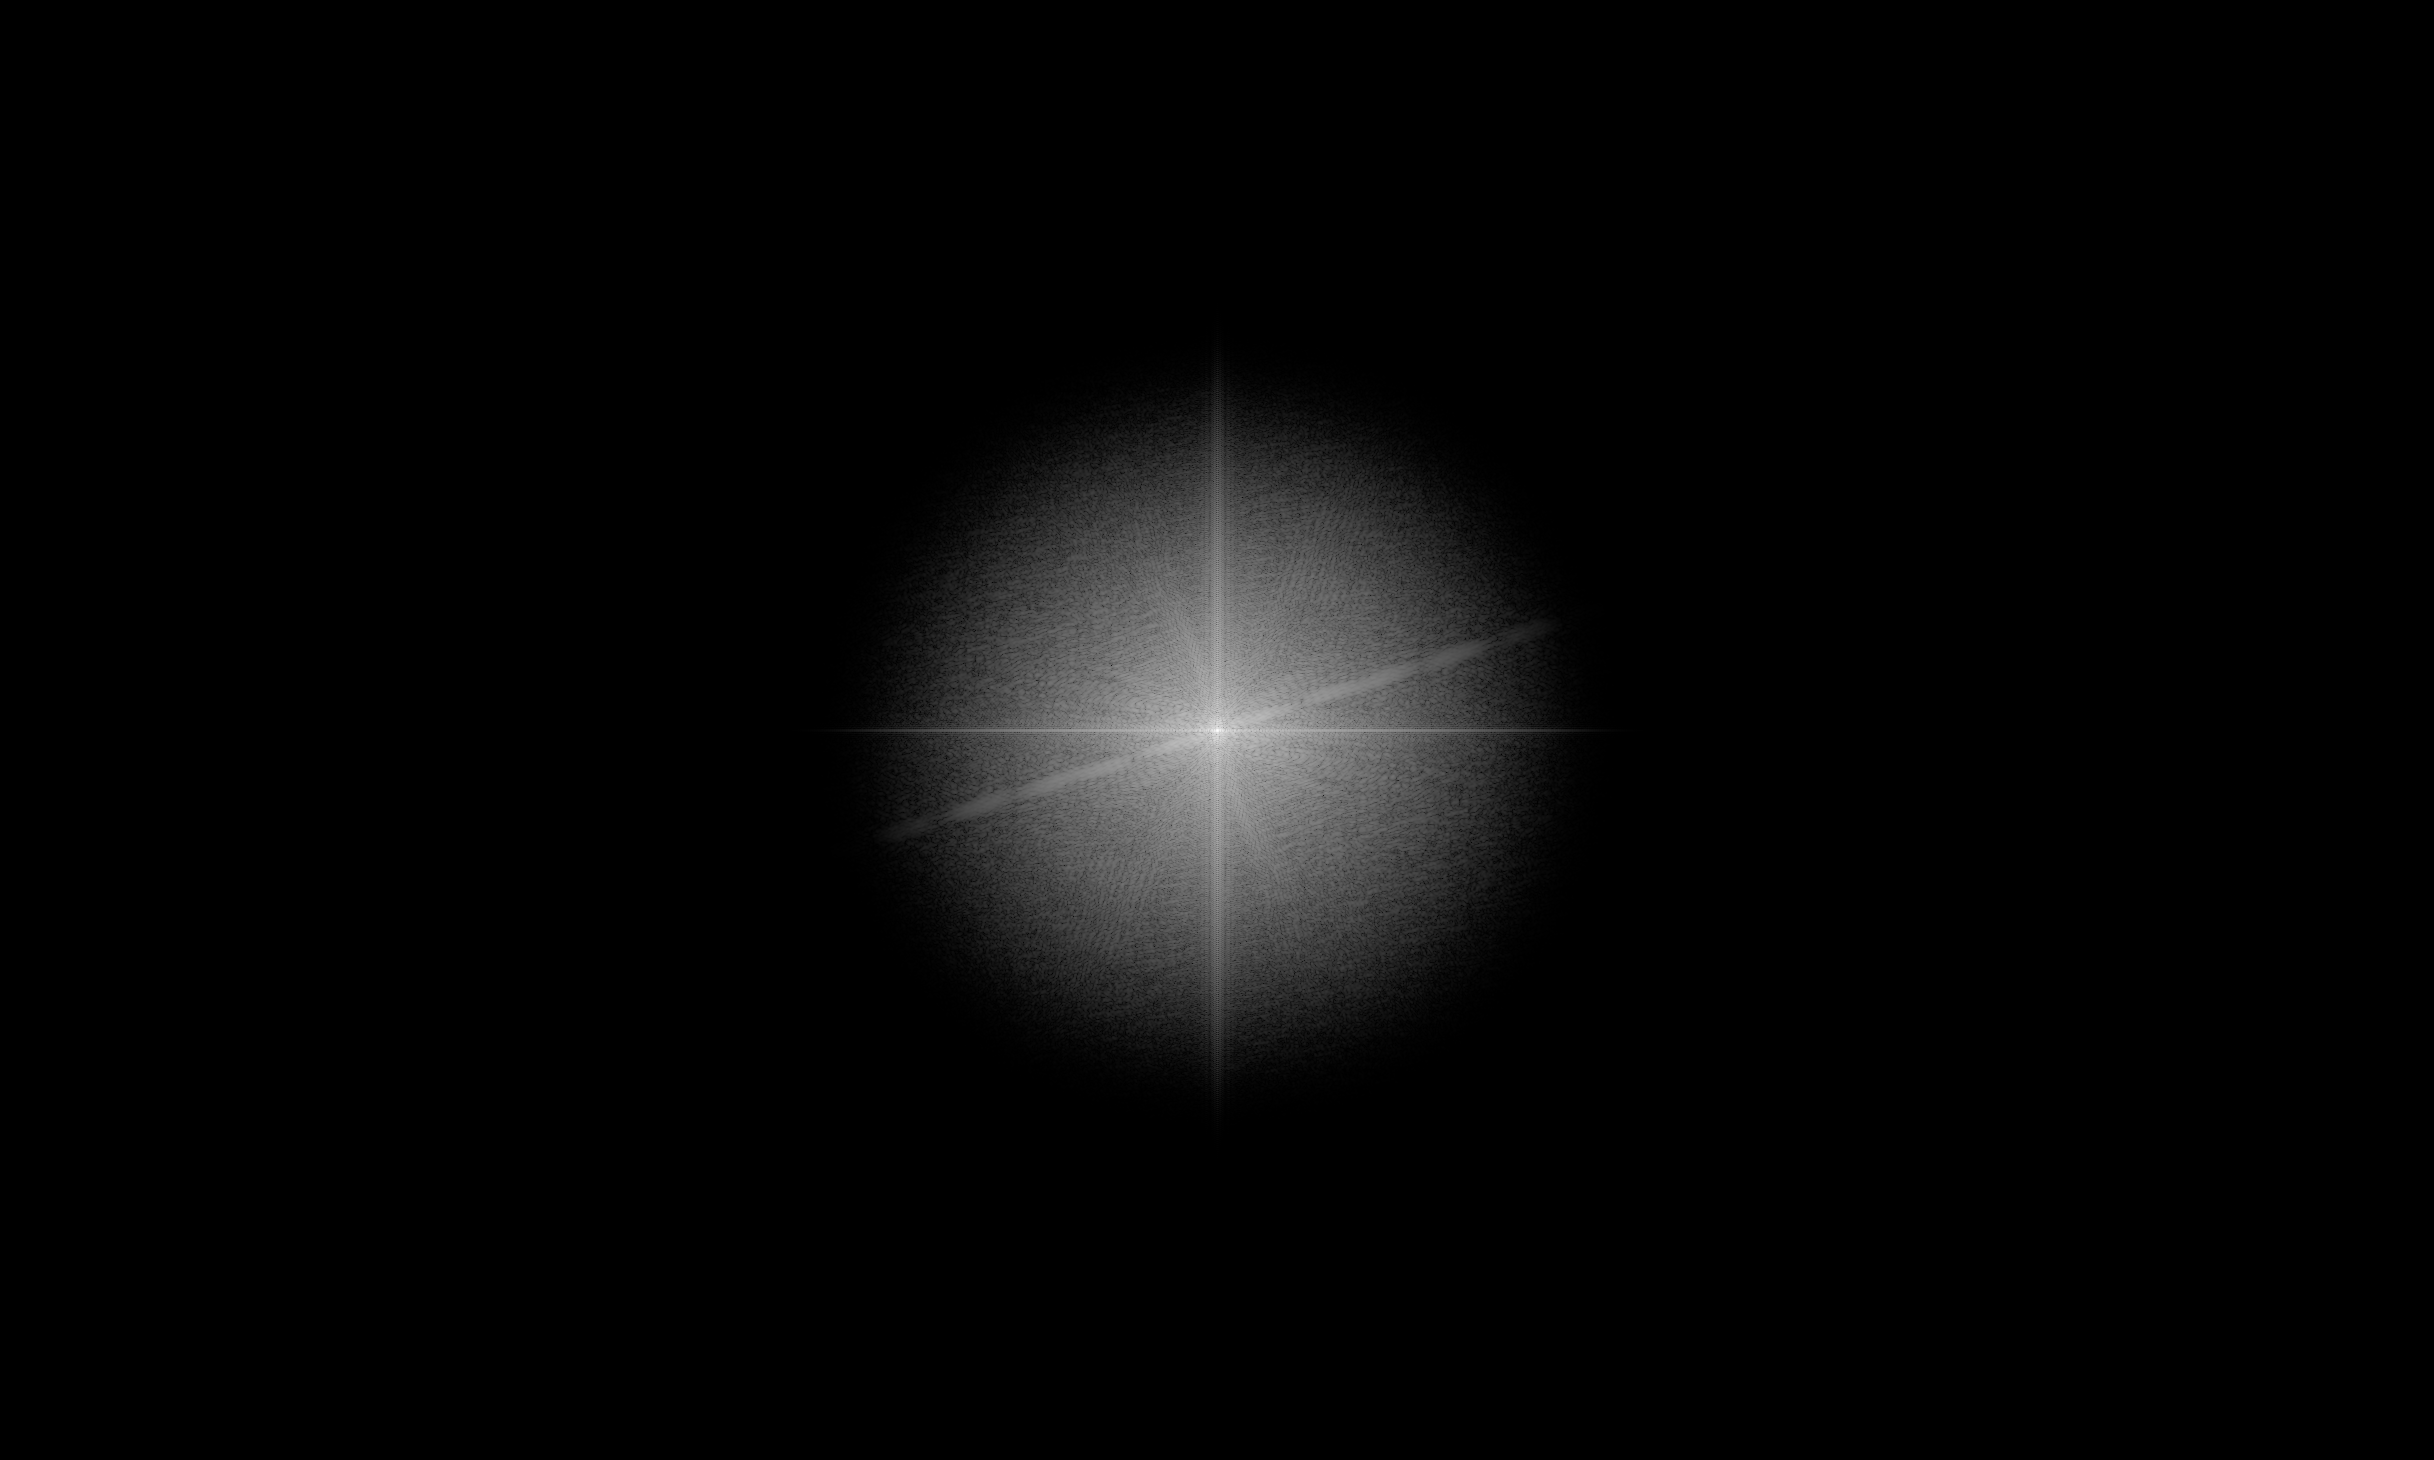
\includegraphics[width=0.47\textwidth]{smooth_result_Gauss//sigma=80 filtered frequency.png}}
    \,    
    \subfigure[滤波效果]
    {\label{} 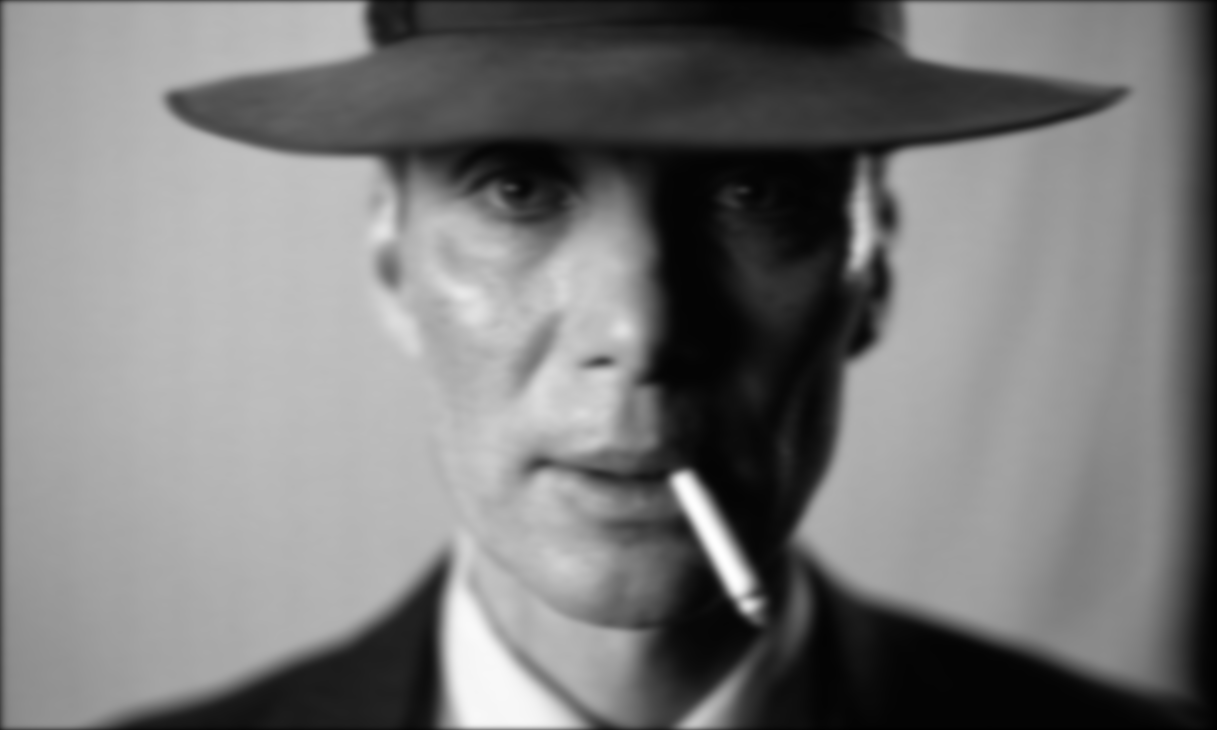
\includegraphics[width=0.47\textwidth]{smooth_result_Gauss//sigma=80 filtered figure.png}}
    \caption{$\sigma=80$的频域低通滤波结果与效果图}\label{} 
\end{figure}


% \paragraph{$\sigma=100$的频域低通滤波结果与效果图}
\begin{figure}[H]
    \centering
    \subfigure[频域低通滤波结果(取对数)]
    {\label{} 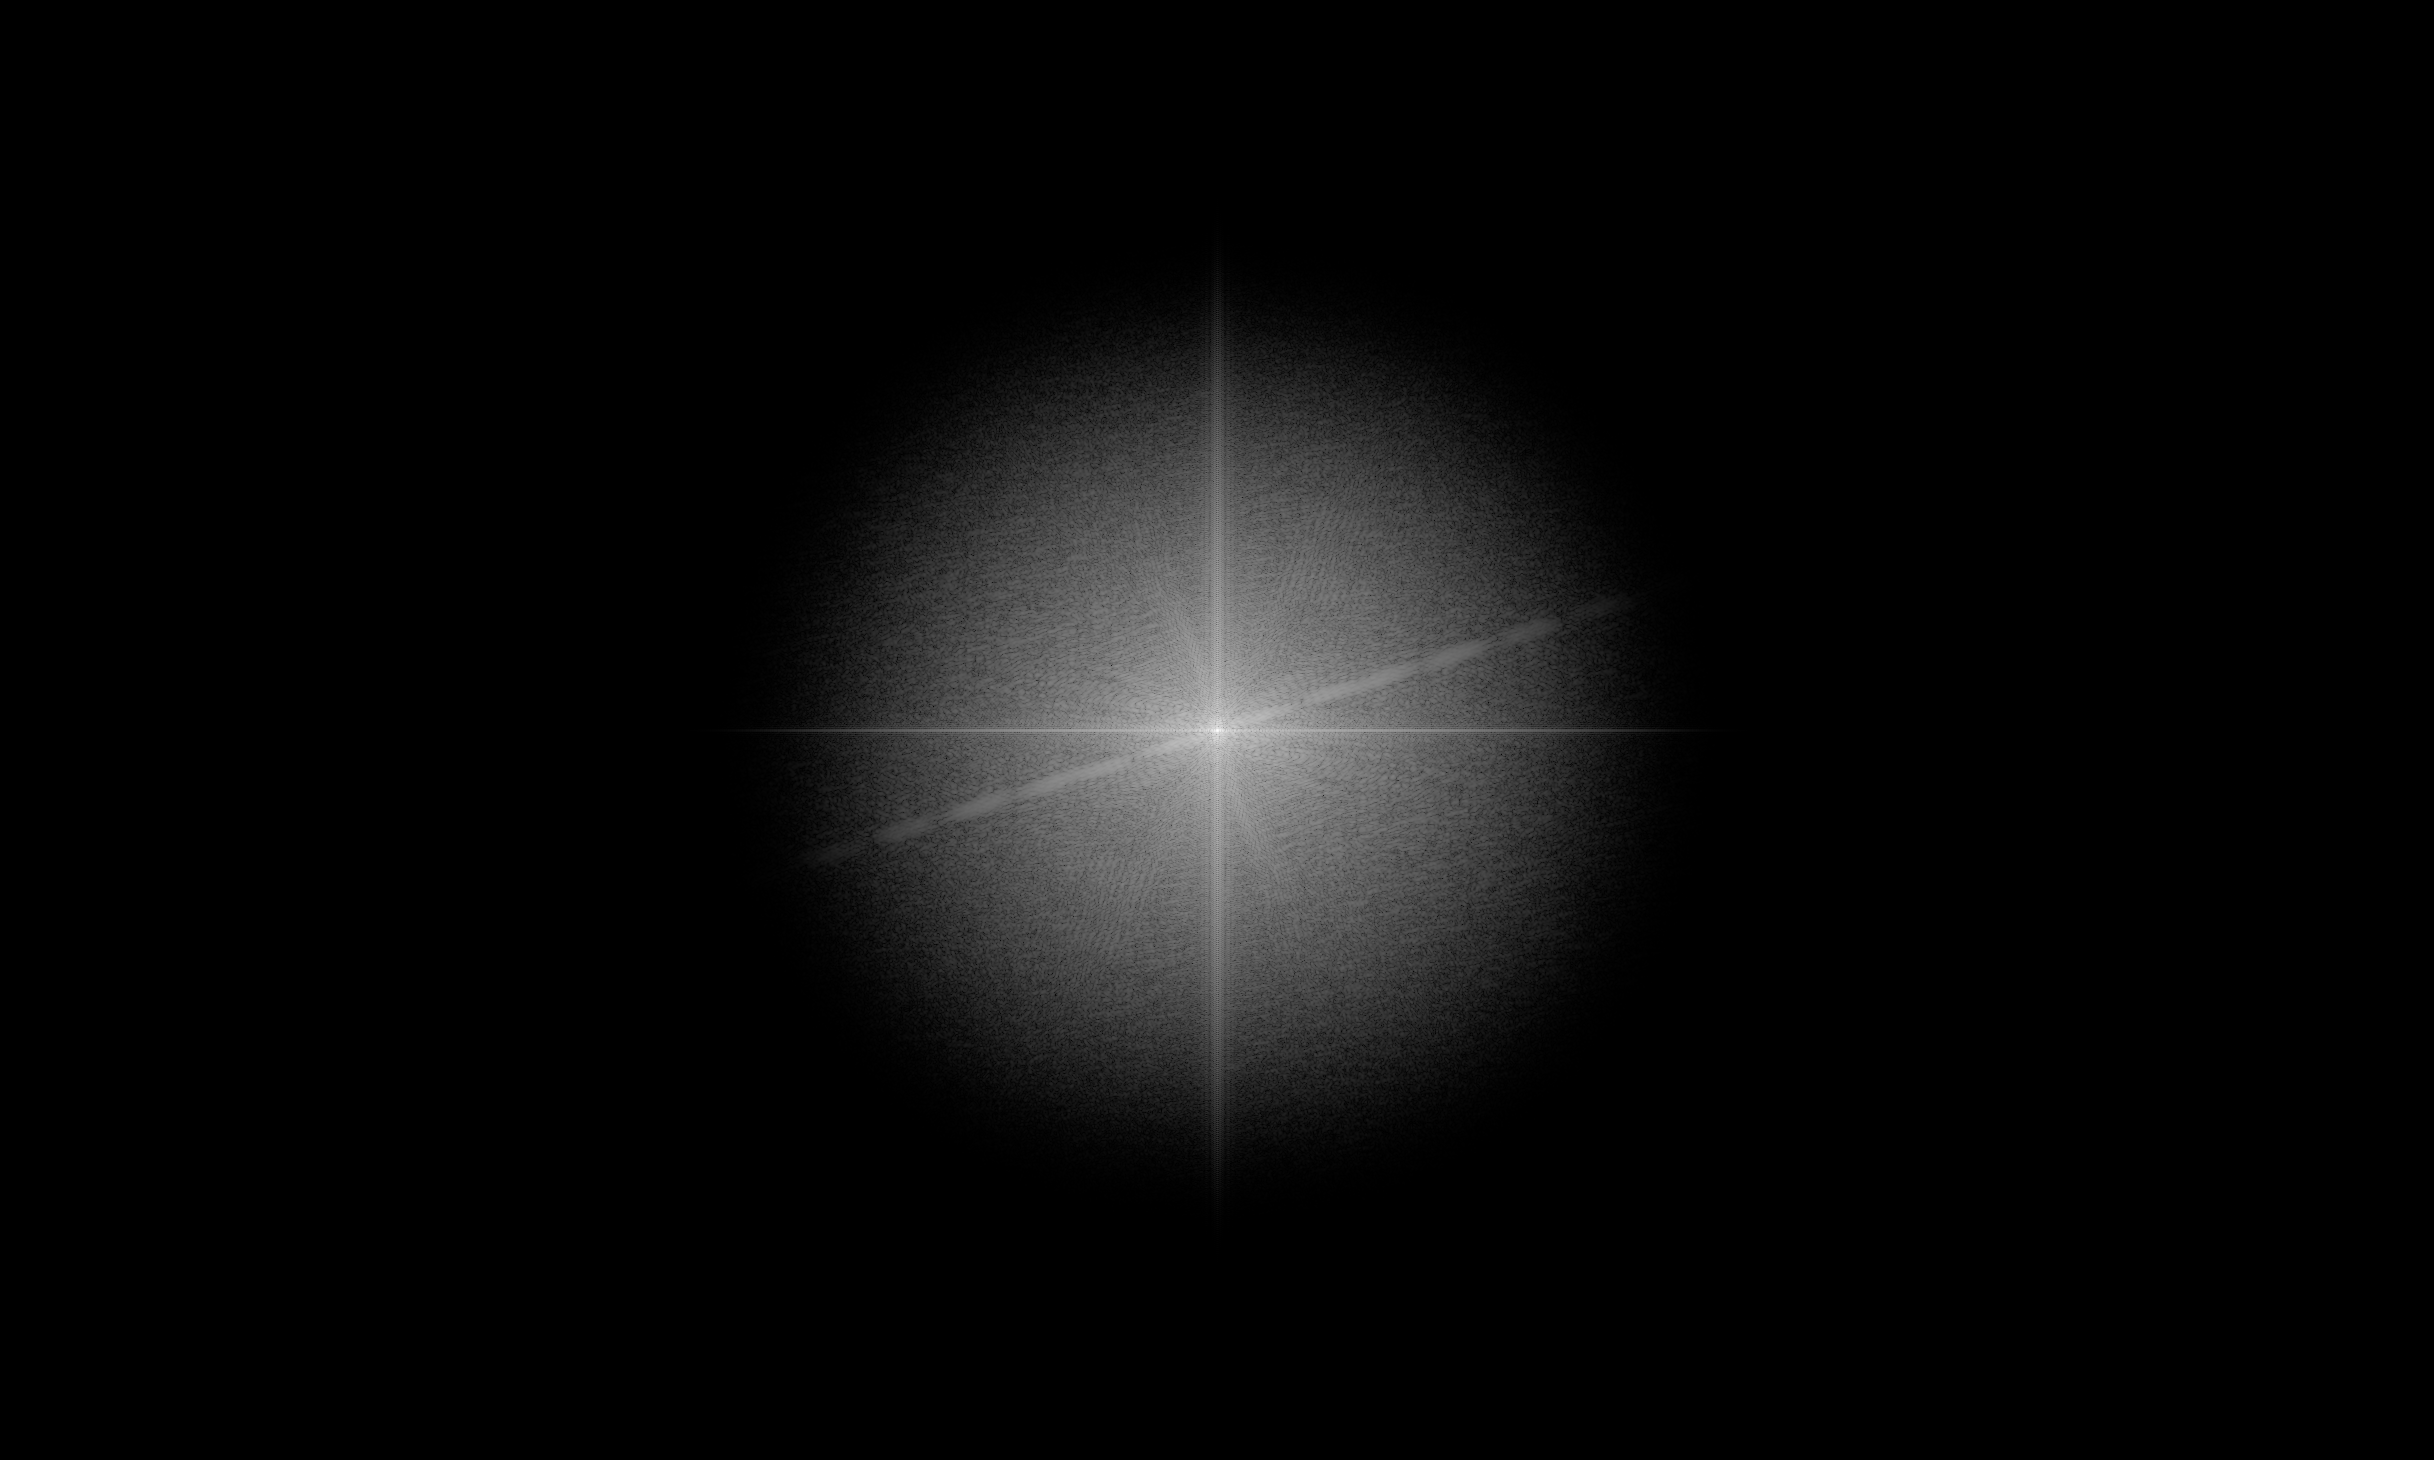
\includegraphics[width=0.47\textwidth]{smooth_result_Gauss//sigma=100 filtered frequency.png}}
    \,    
    \subfigure[滤波效果]
    {\label{} 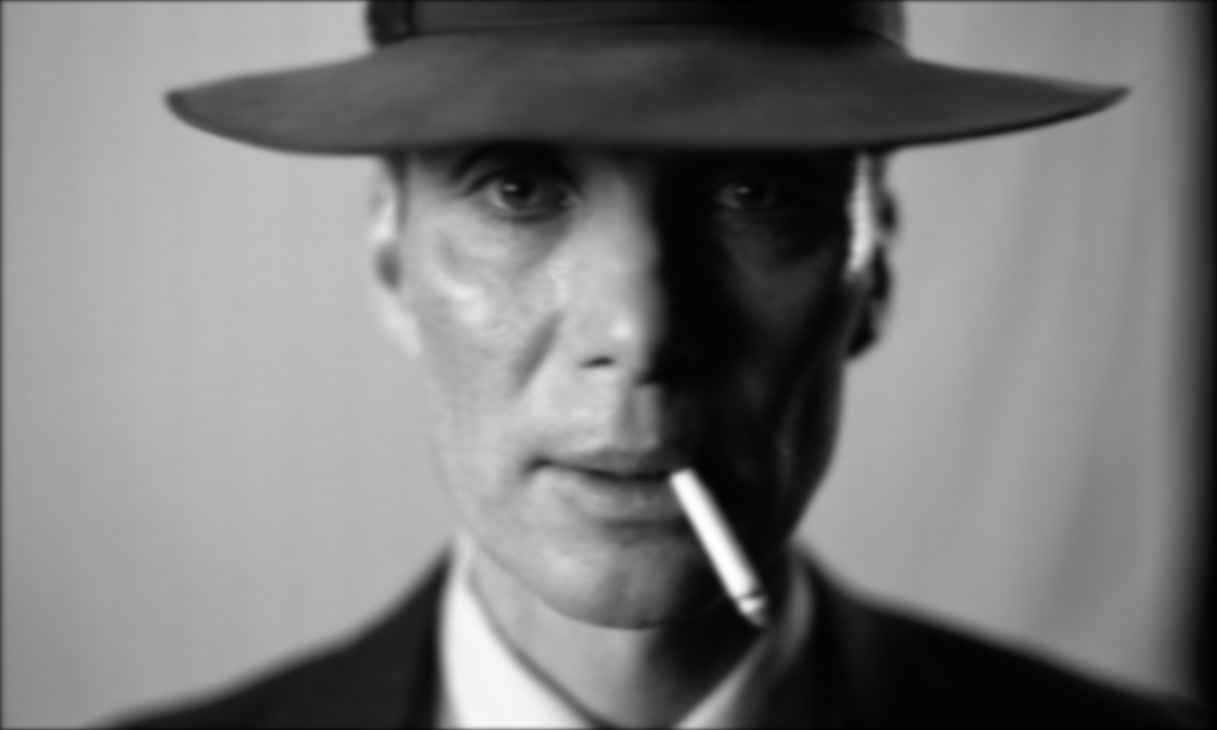
\includegraphics[width=0.47\textwidth]{smooth_result_Gauss//sigma=100 filtered figure.png}}
    \caption{$\sigma=100$的频域低通滤波结果与效果图}\label{} 
\end{figure}

\paragraph{小结}
可以明显看出,\textbf{$\sigma$越小,平滑的效果越好}。

\subsection{锐化}

\subsubsection{频域滤波器:高斯高通滤波器(GHPF)}
使用的高斯高通滤波器如下

\[
H(u,v) = 1 - \exp[-D^2(u,v)/2\sigma^2]	+ c
\]
其中
\[
D^2(u,v) = (u-u_0)^2 + (v-v_0)^2	
\]
$(u_0,v_0)$ 表示频域的中心点,$\sigma$表示高斯滤波器的标准差,$\sigma$越大,
去除的低频信号就会越多。$c$是一个常数,在本次实验中统一取$c=1$,该常数不会影响锐化效果,
同时能保留原始的整体灰度值信息,使得滤波后的图像色调与原图尽可能一直。

\subsubsection{Python代码实现}

实现锐化的Python代码如下,其中,\textbf{频域滤波的五个标准步骤都已经写在sharpen函数的注释中},
敬请读者结合代码进行审阅。

\lstinputlisting[style = Python,
caption={Python codes for sharpening by GHPF},
label = {GHPF}]{1_2_sharpen_GHPF.py}


\subsubsection{效果展示}
仍然使用平滑操作中的图\ref{ori.sub.1}作为测试用图。不同的$\sigma$对应锐化效果如下

% \paragraph{$\sigma=1$的频域高通滤波结果与效果图}
\begin{figure}[H]
    \centering
    \subfigure[频域高通滤波结果(取对数)]
    {\label{} 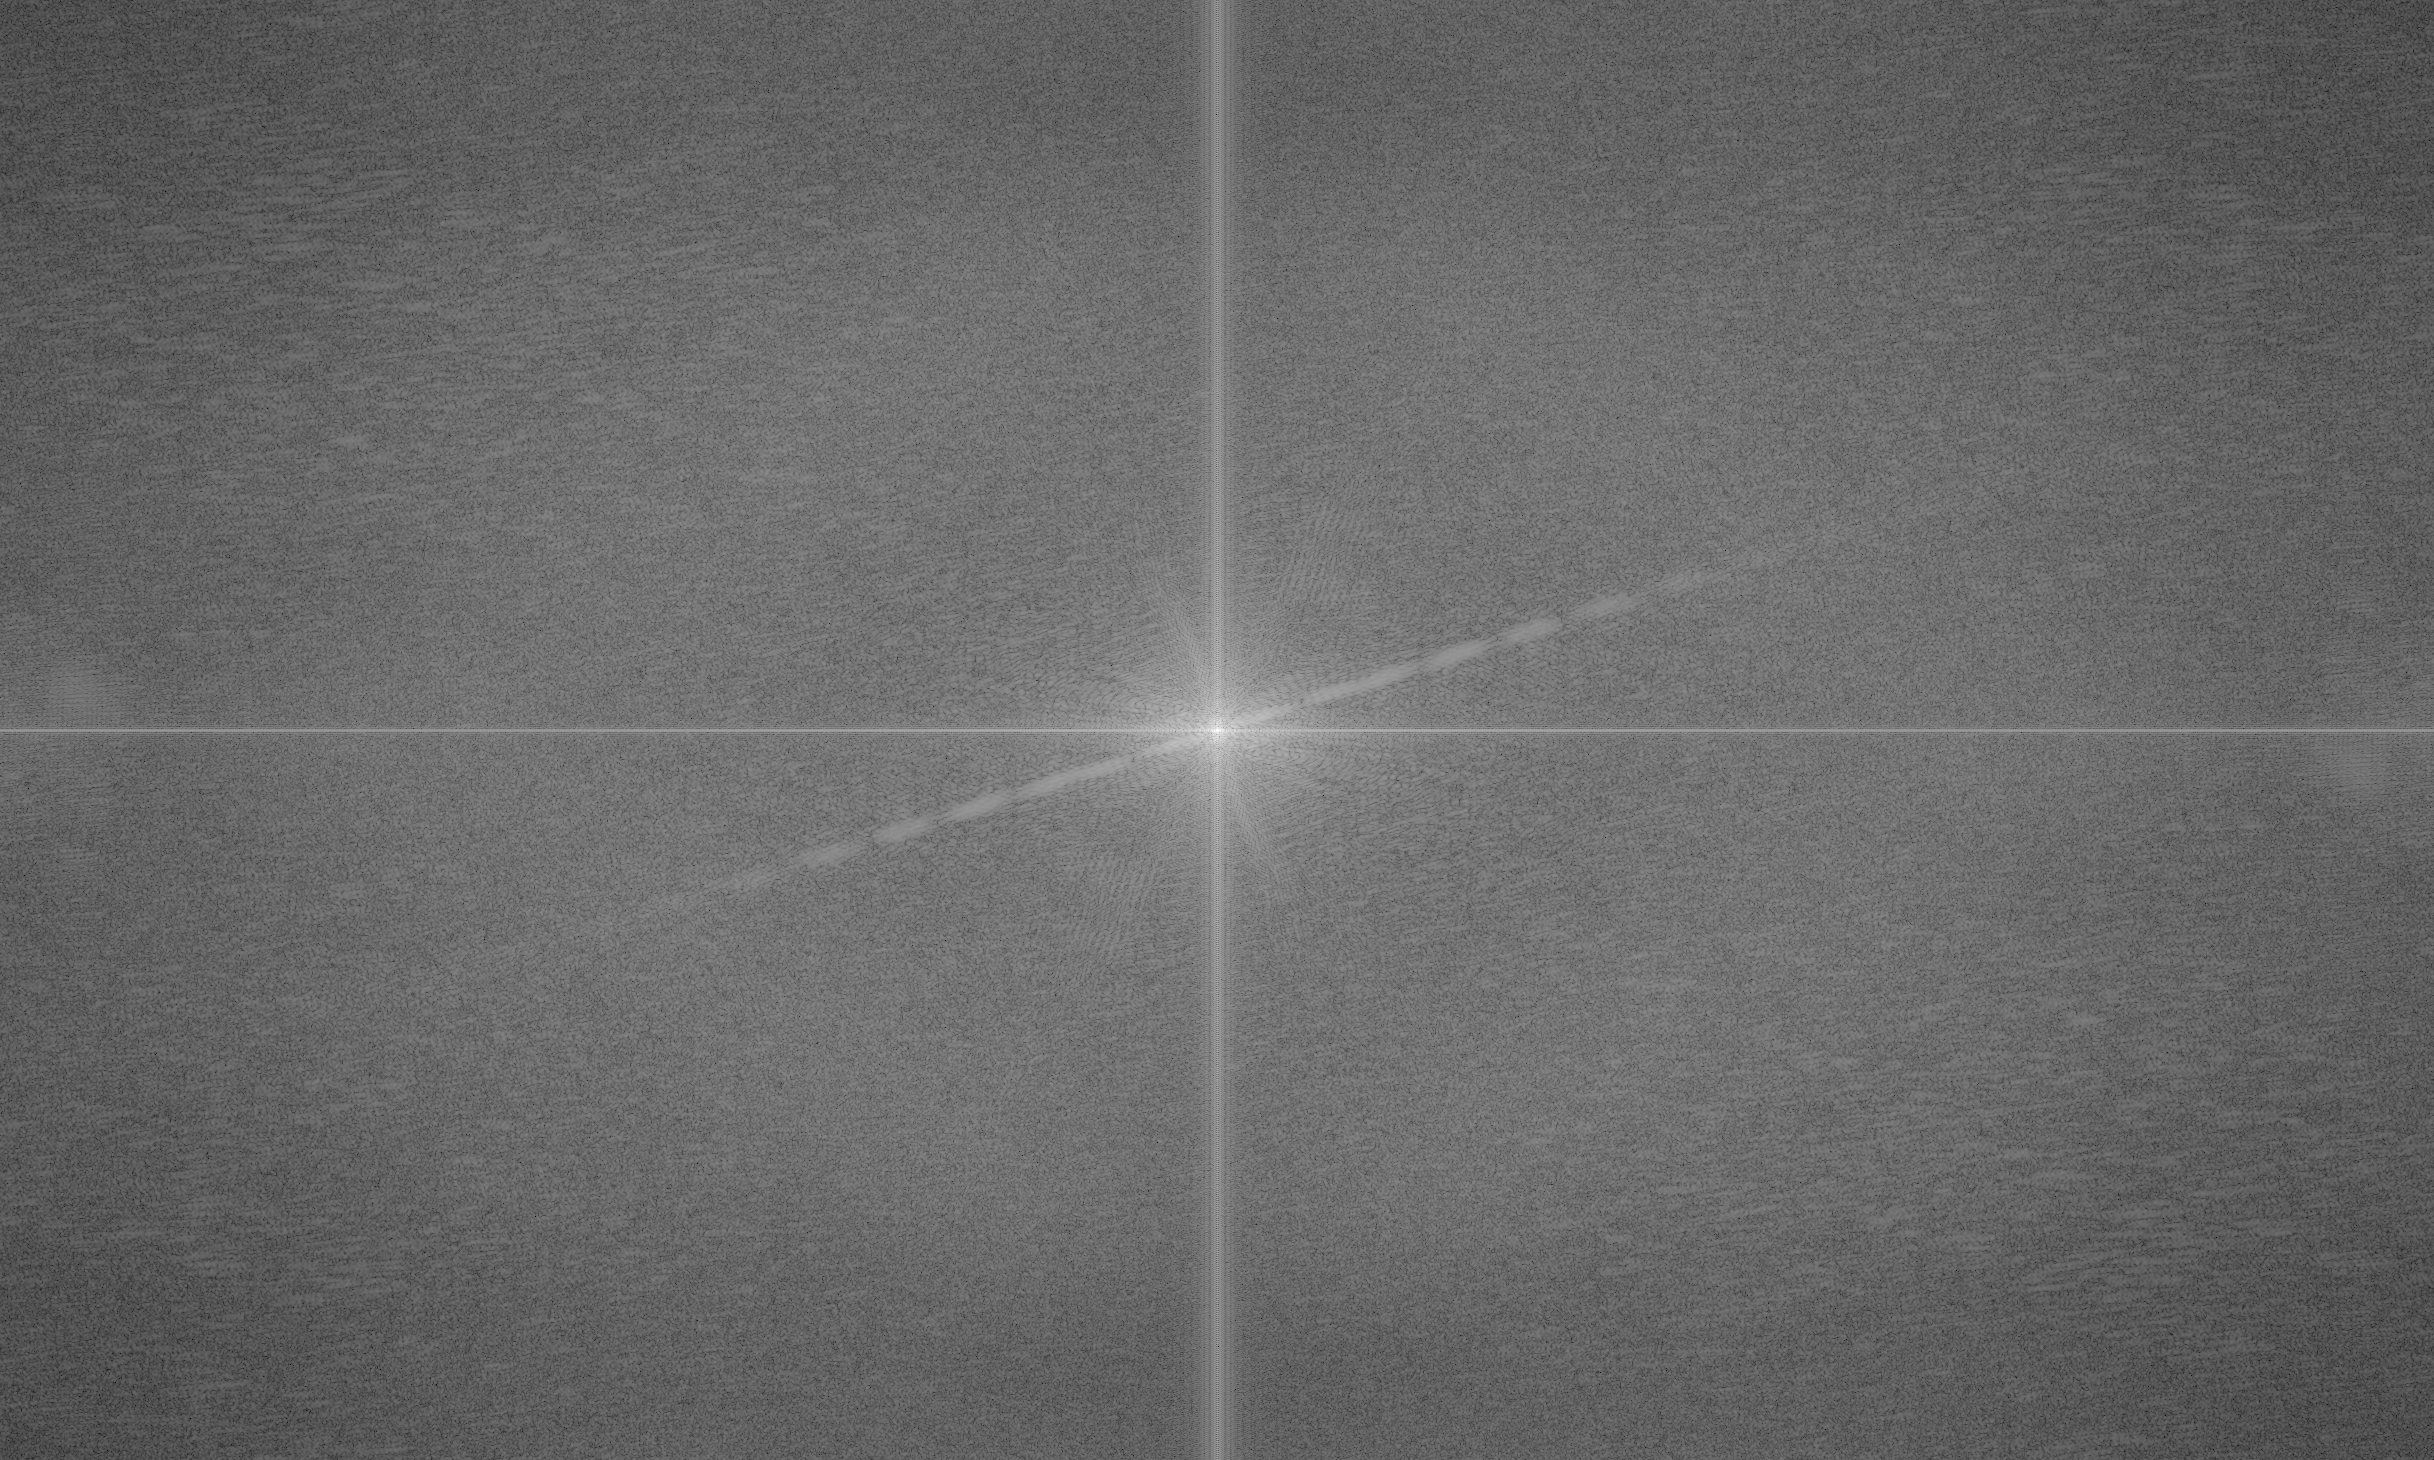
\includegraphics[width=0.47\textwidth]{sharpen_result_Gauss//sigma=1 c=1 filtered frequency.png}}
    \,    
    \subfigure[滤波效果]
    {\label{} 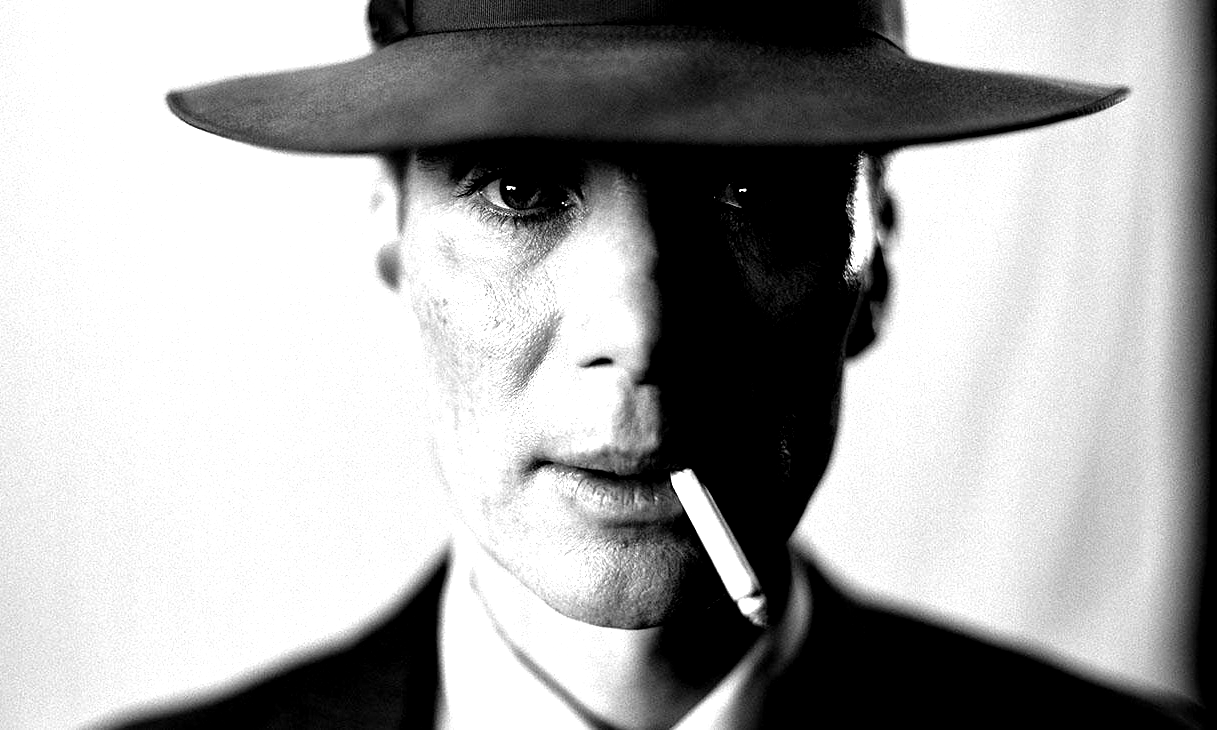
\includegraphics[width=0.47\textwidth]{sharpen_result_Gauss//sigma=1 c=1 filtered figure.png}}
    \caption{$\sigma=1$的频域高通滤波结果与效果图}\label{} 
\end{figure}


% \paragraph{$\sigma=2$的频域高通滤波结果与效果图}
\begin{figure}[H]
    \centering
    \subfigure[频域高通滤波结果(取对数)]
    {\label{} 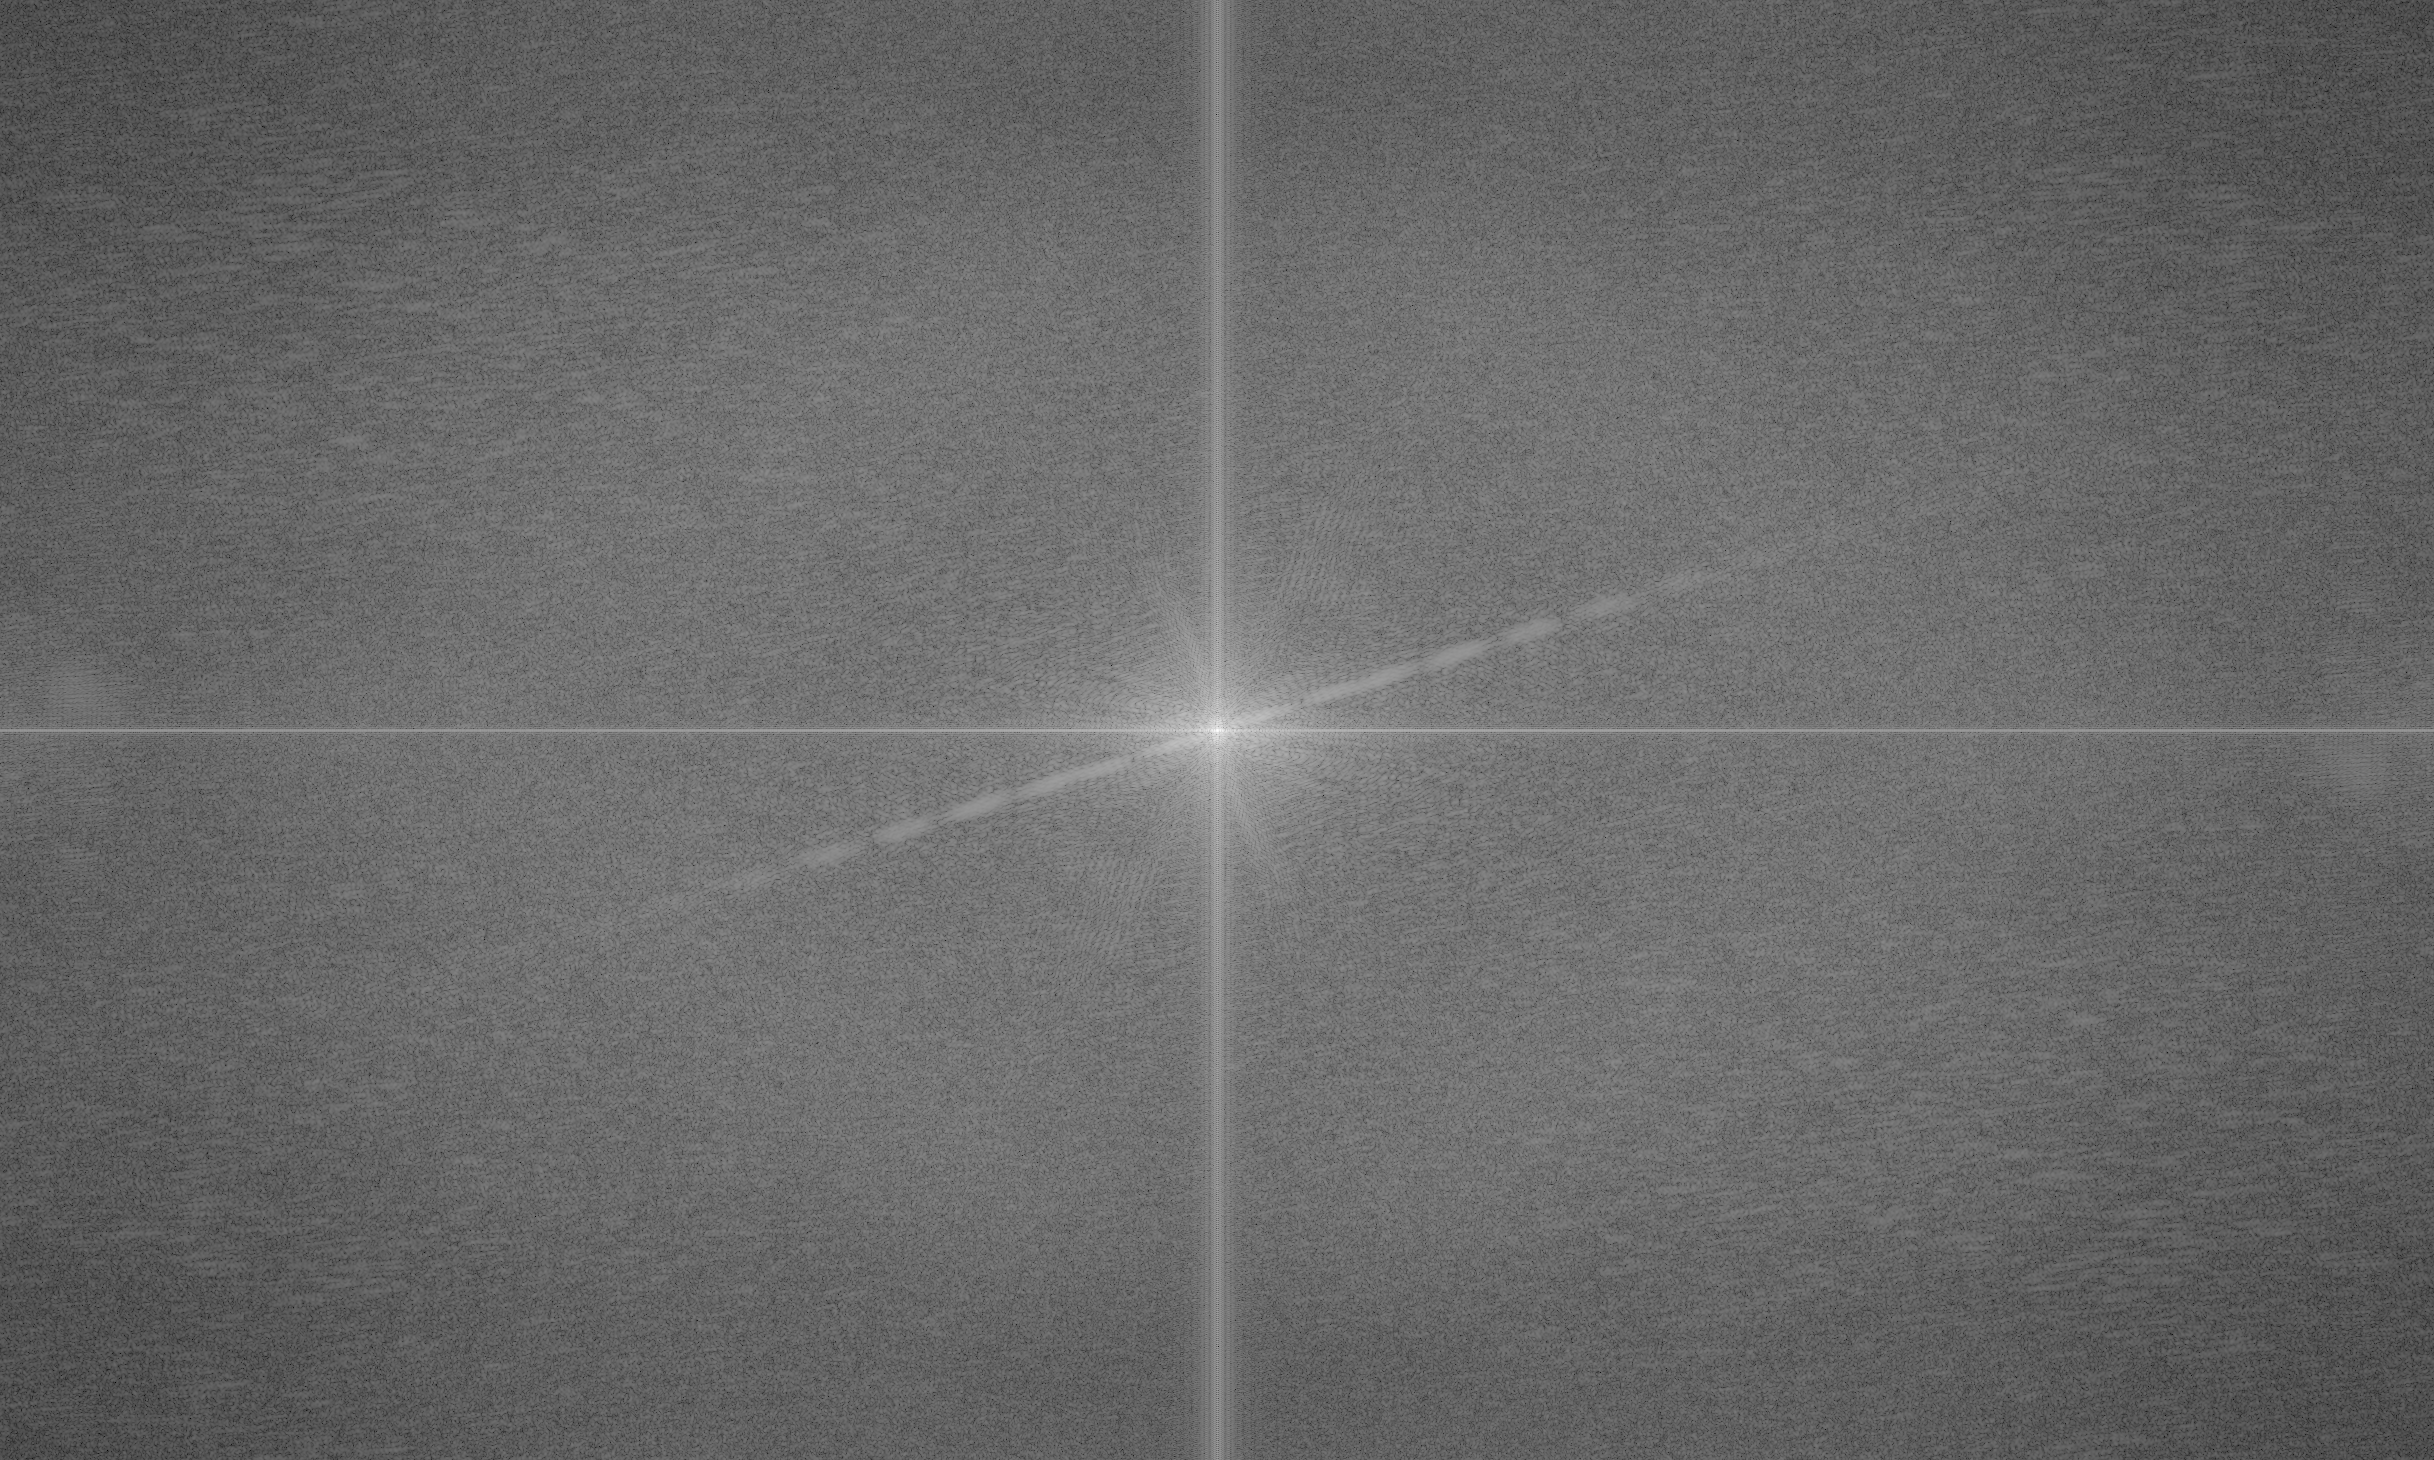
\includegraphics[width=0.47\textwidth]{sharpen_result_Gauss//sigma=2 c=1 filtered frequency.png}}
    \,    
    \subfigure[滤波效果]
    {\label{} 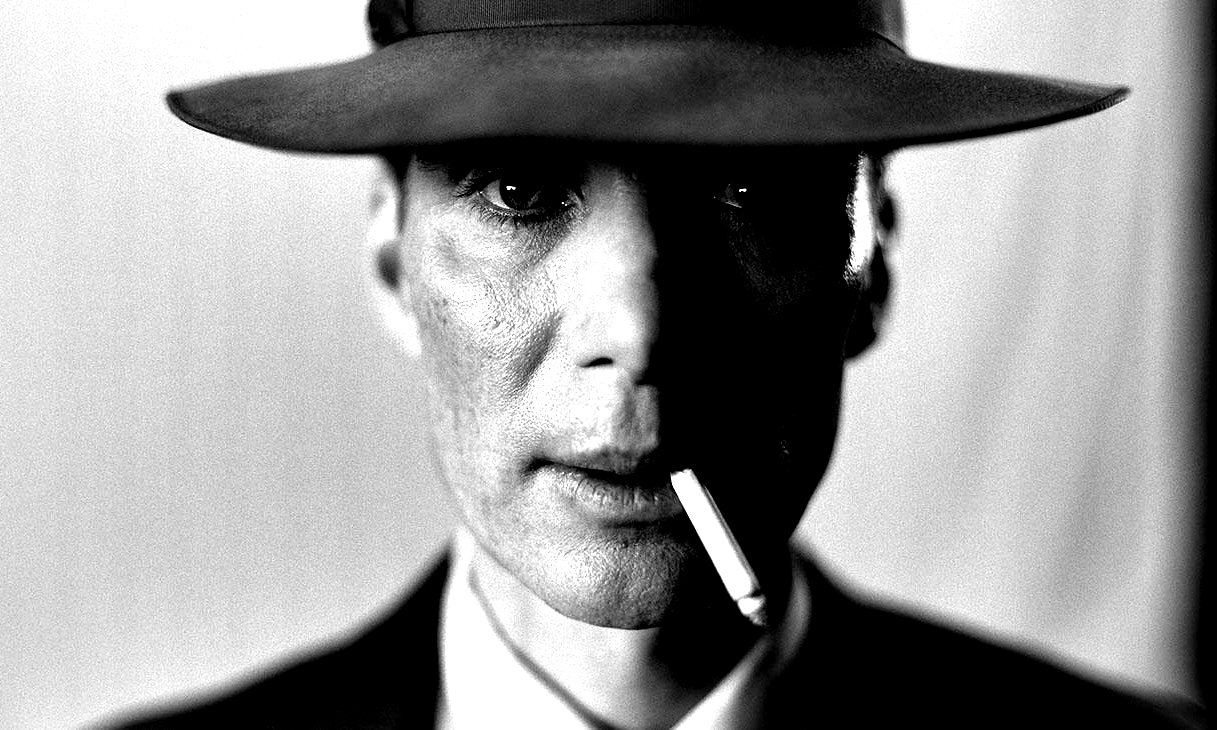
\includegraphics[width=0.47\textwidth]{sharpen_result_Gauss//sigma=2 c=1 filtered figure.png}}
    \caption{$\sigma=2$的频域高通滤波结果与效果图}\label{} 
\end{figure}


% \paragraph{$\sigma=5$的频域高通滤波结果与效果图}
\begin{figure}[H]
    \centering
    \subfigure[频域高通滤波结果(取对数)]
    {\label{} 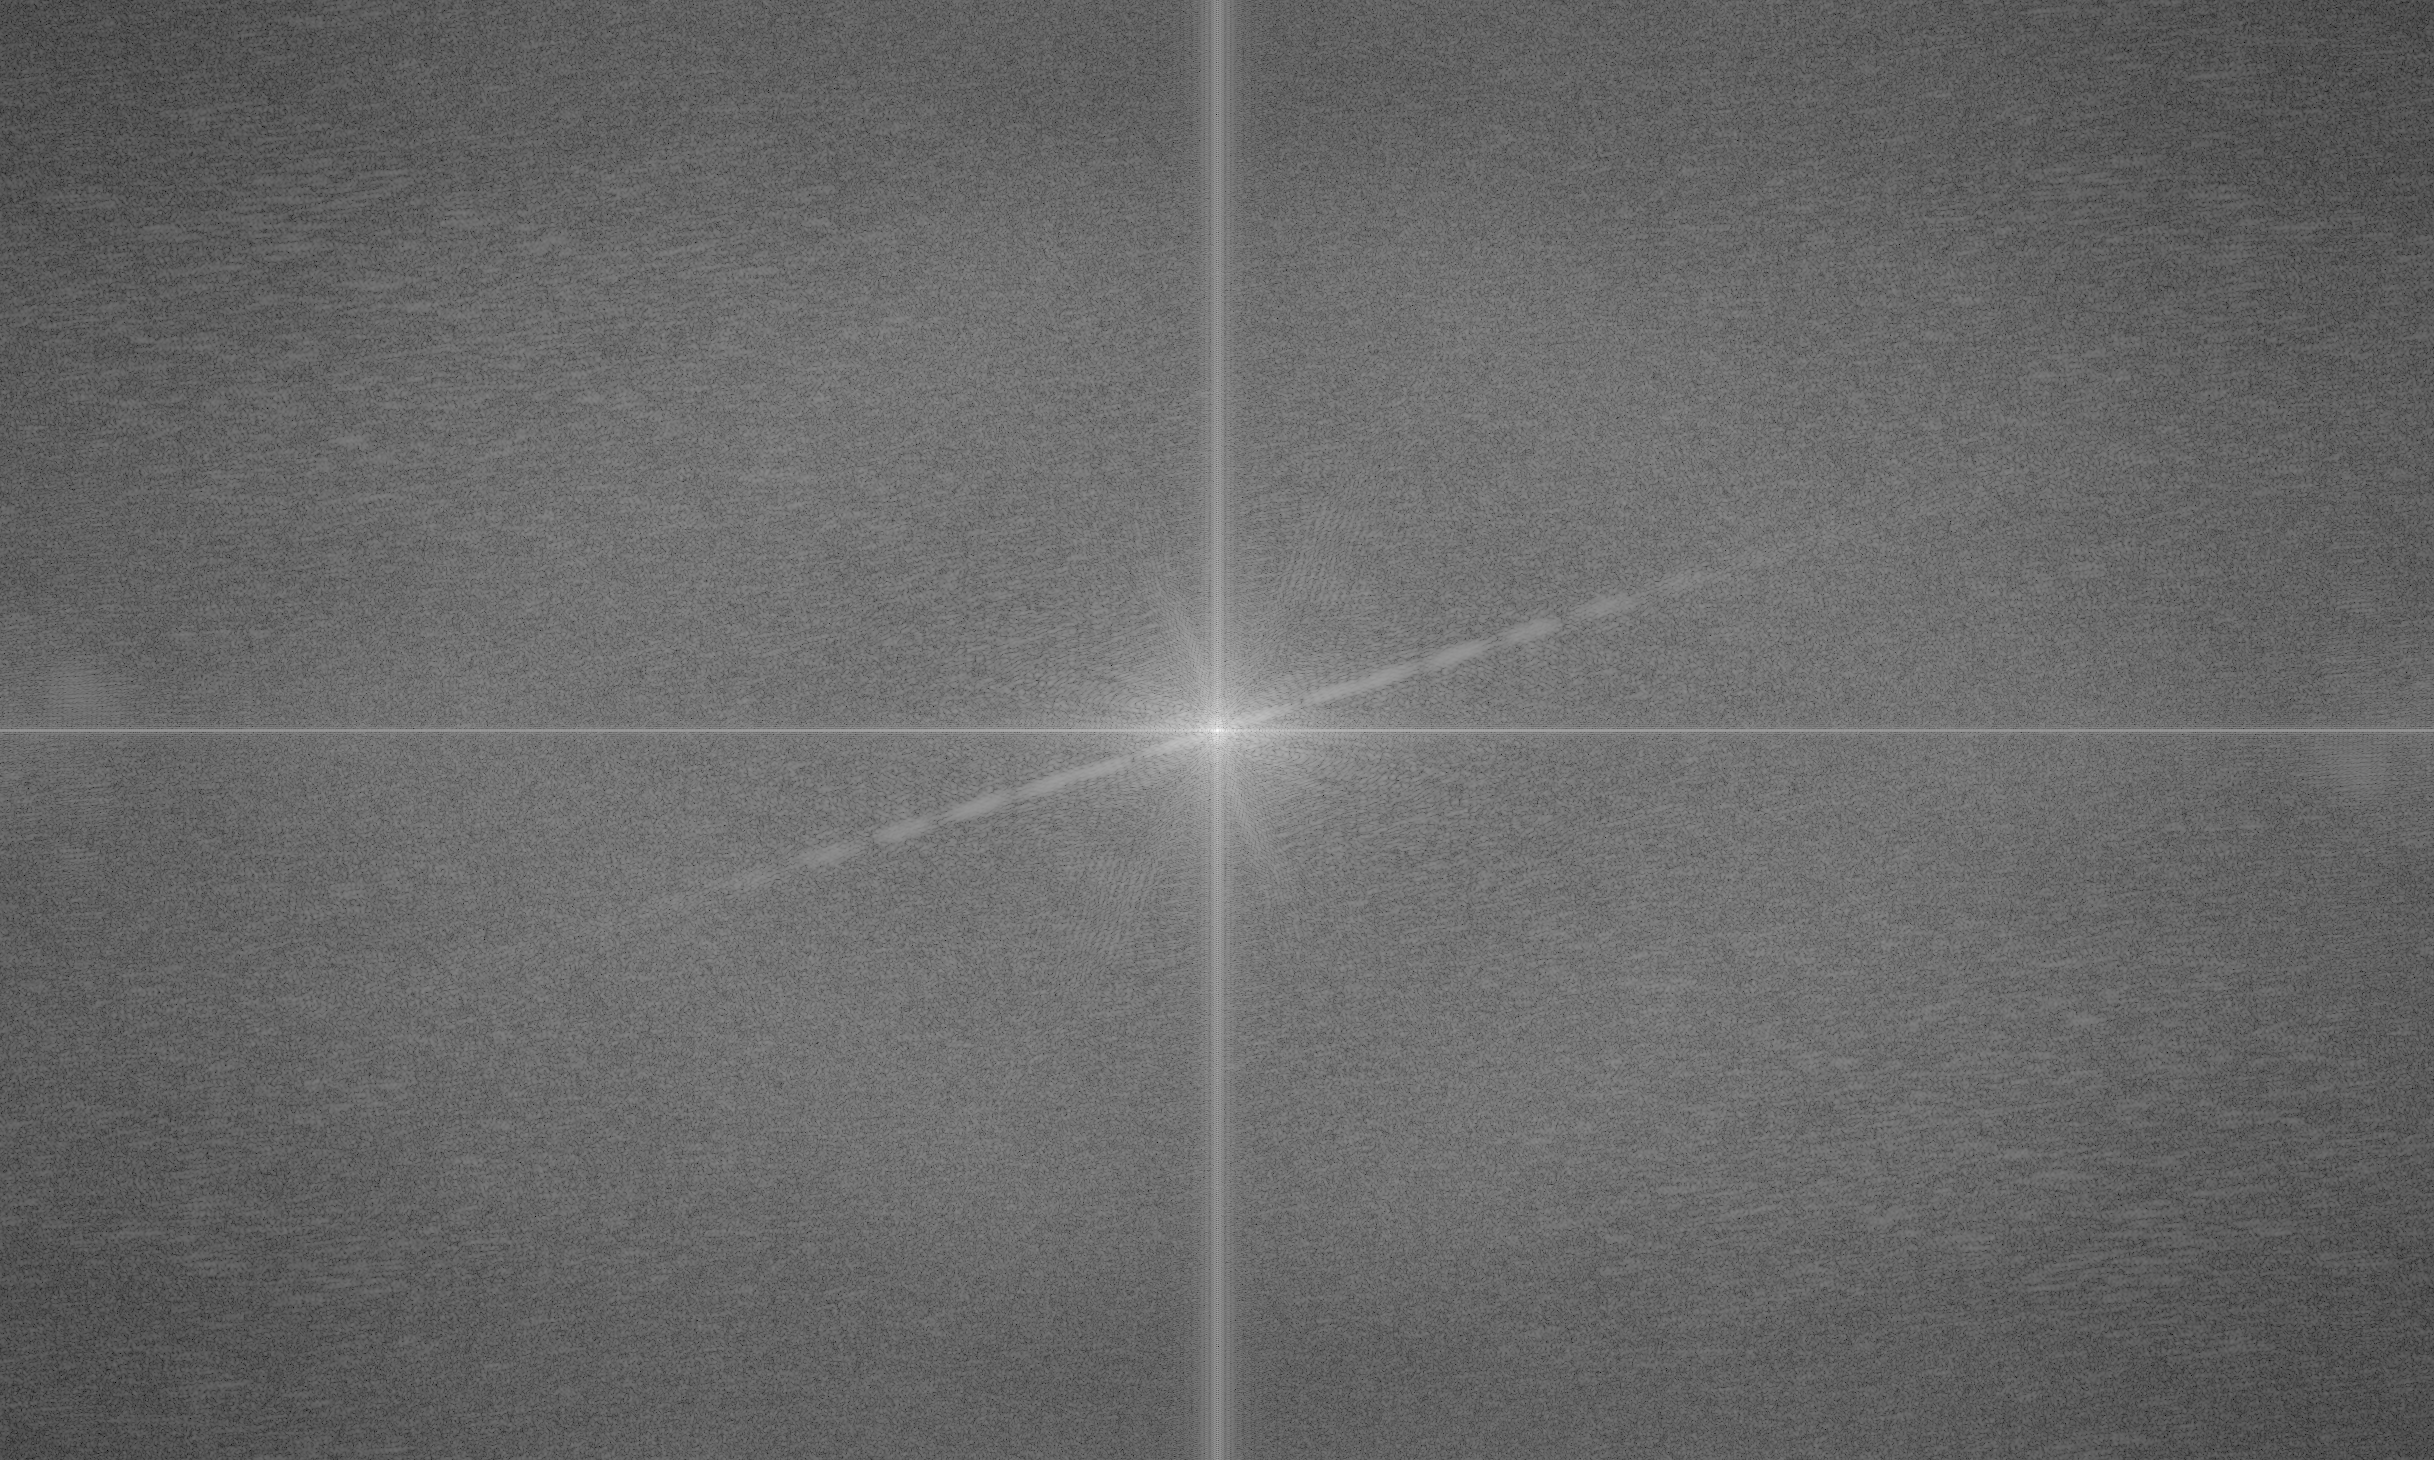
\includegraphics[width=0.47\textwidth]{sharpen_result_Gauss//sigma=5 c=1 filtered frequency.png}}
    \,    
    \subfigure[滤波效果]
    {\label{} 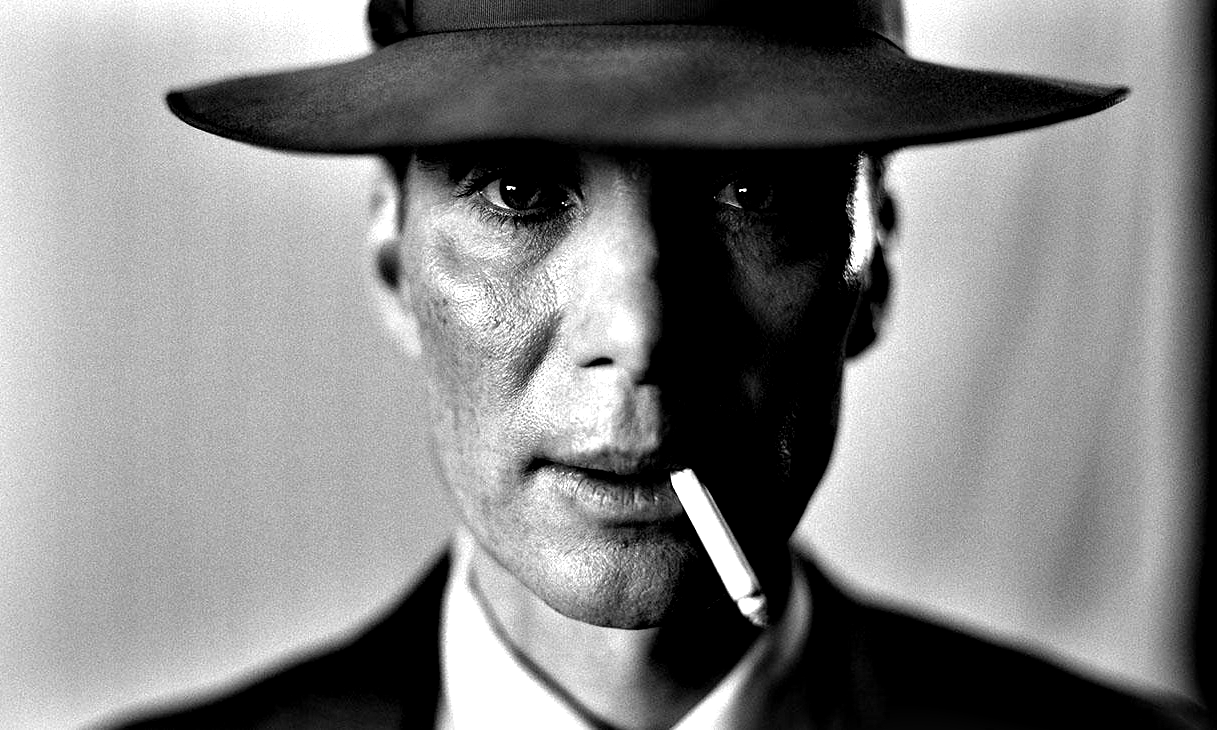
\includegraphics[width=0.47\textwidth]{sharpen_result_Gauss//sigma=5 c=1 filtered figure.png}}
    \caption{$\sigma=5$的频域高通滤波结果与效果图}\label{} 
\end{figure}



% \paragraph{$\sigma=10$的频域高通滤波结果与效果图}
\begin{figure}[H]
    \centering
    \subfigure[频域高通滤波结果(取对数)]
    {\label{} 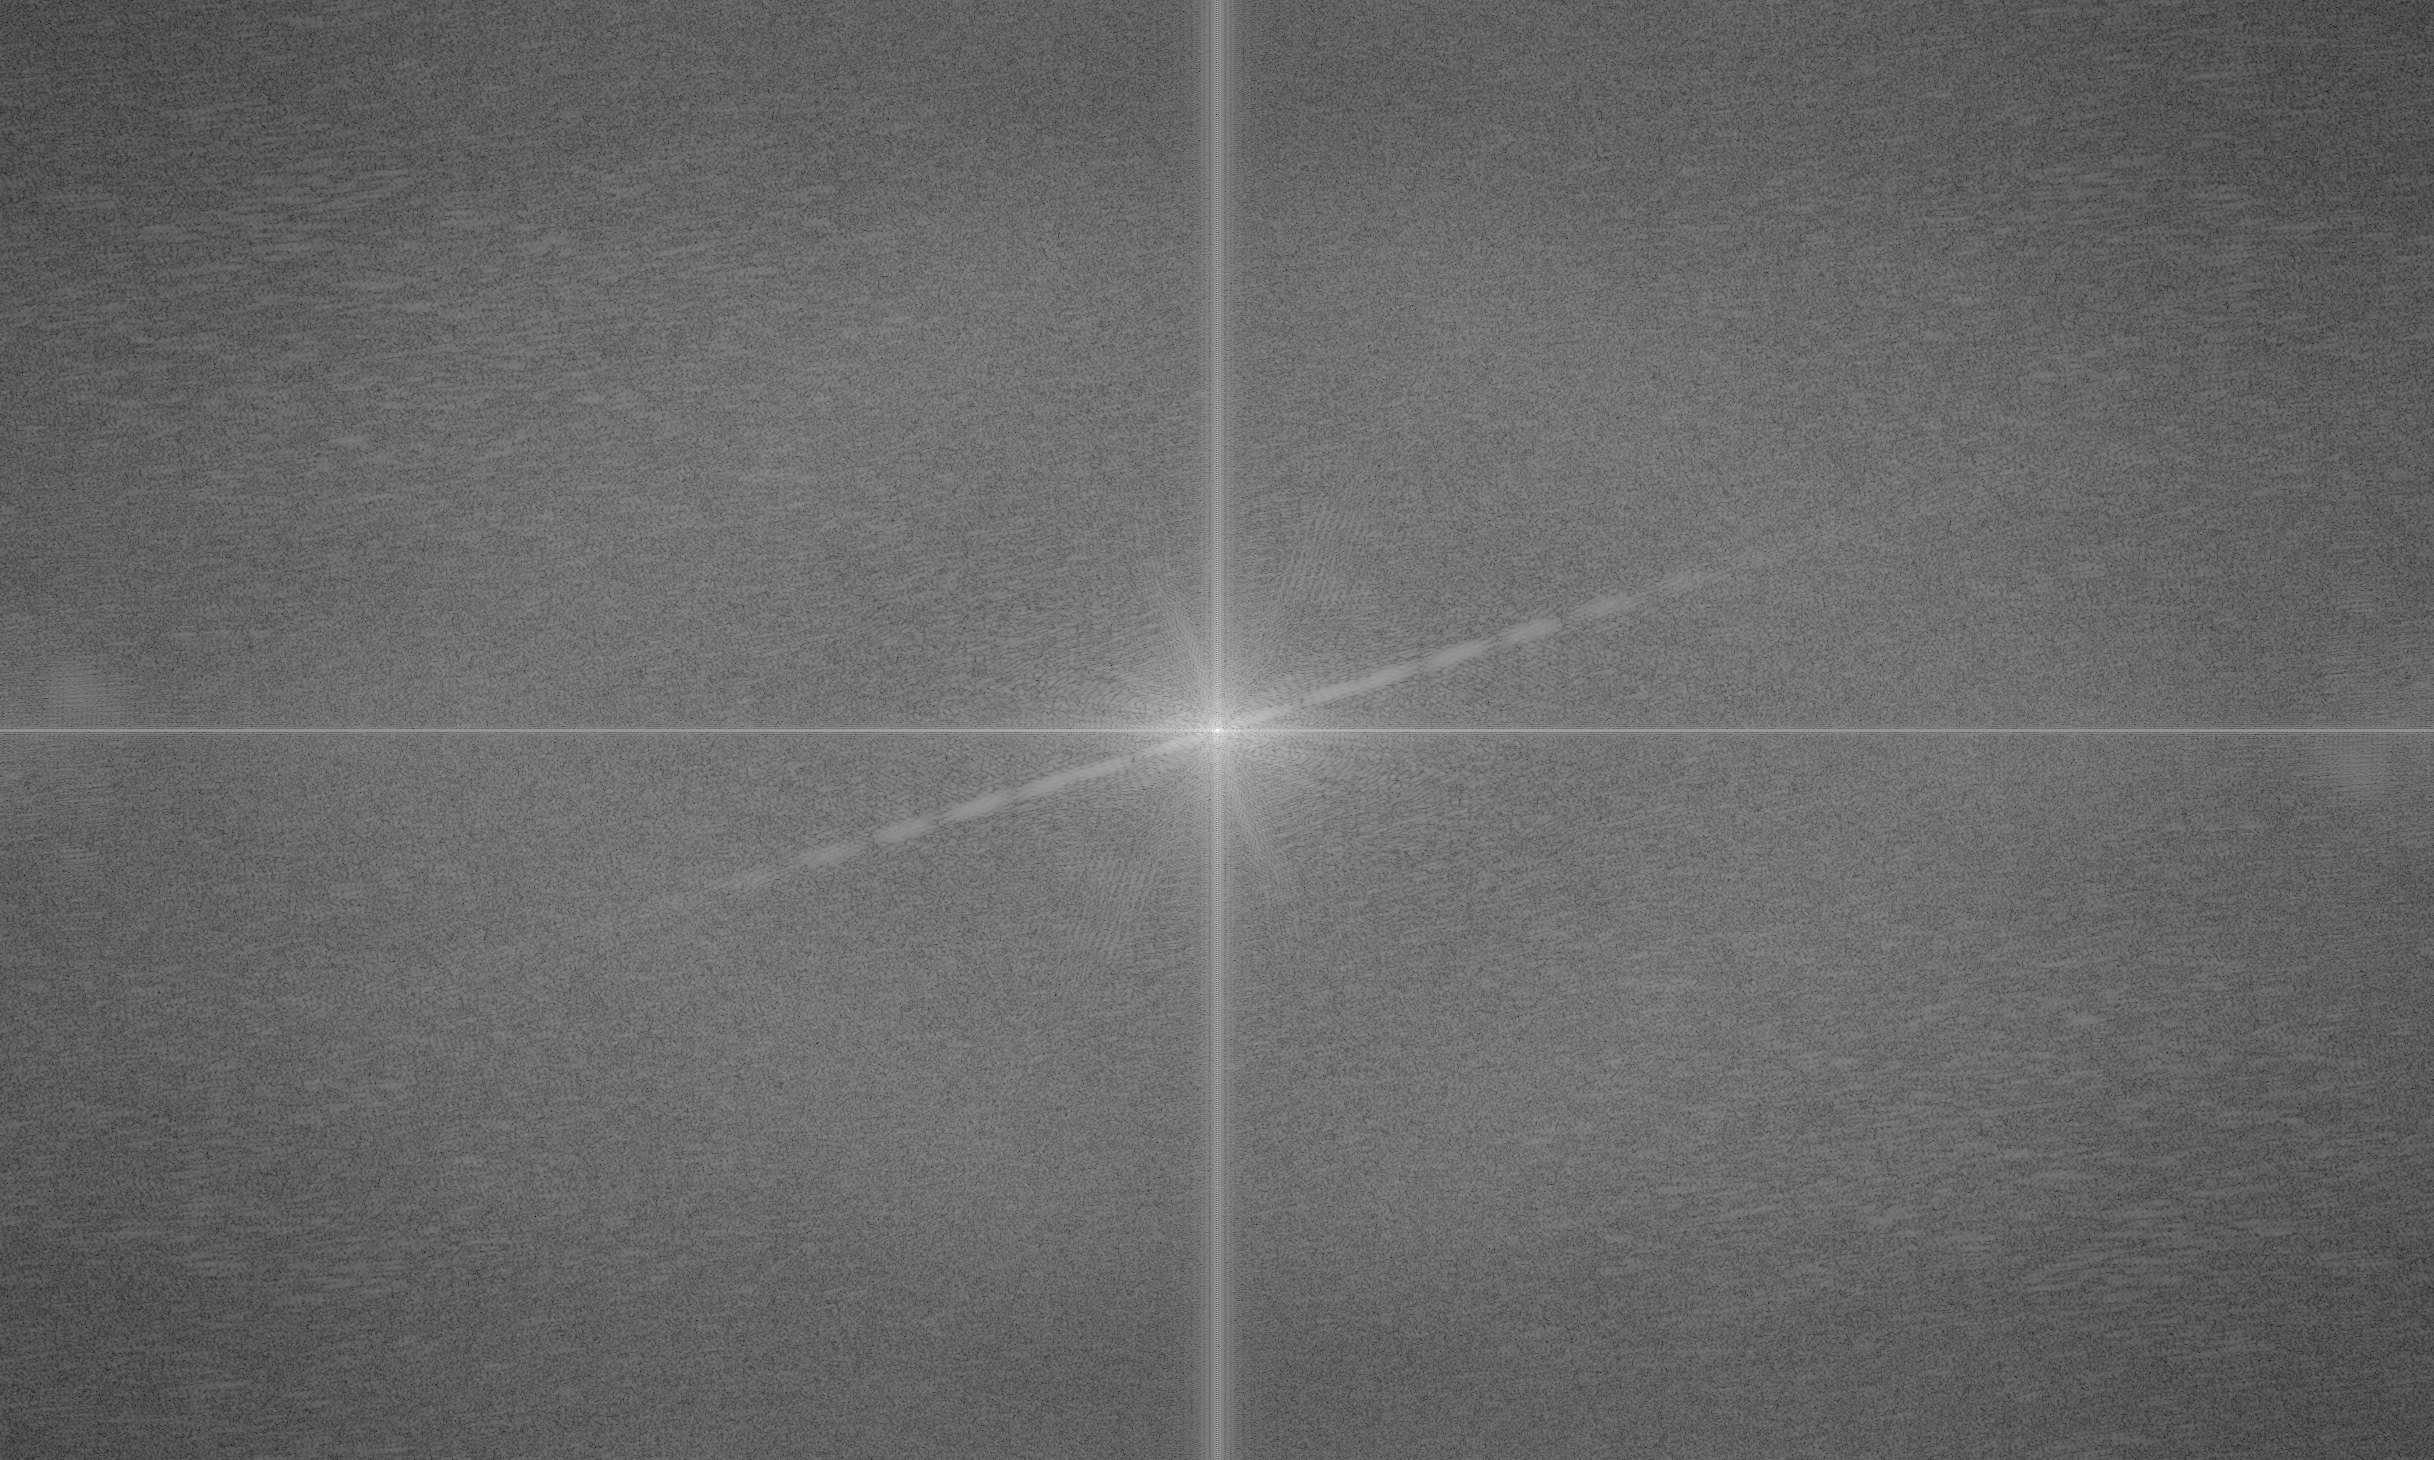
\includegraphics[width=0.47\textwidth]{sharpen_result_Gauss//sigma=10 c=1 filtered frequency.png}}
    \,    
    \subfigure[滤波效果]
    {\label{} 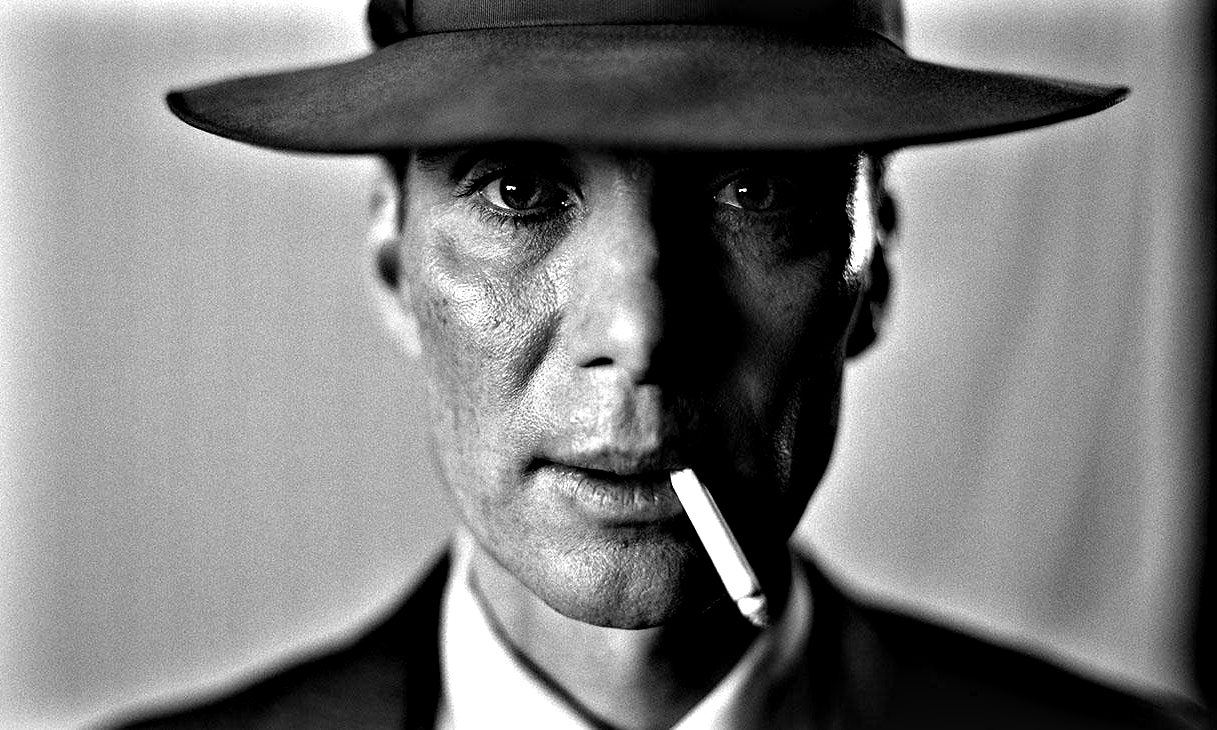
\includegraphics[width=0.47\textwidth]{sharpen_result_Gauss//sigma=10 c=1 filtered figure.png}}
    \caption{$\sigma=10$的频域高通滤波结果与效果图}\label{} 
\end{figure}


% \paragraph{$\sigma=20$的频域高通滤波结果与效果图}
\begin{figure}[H]
    \centering
    \subfigure[频域高通滤波结果(取对数)]
    {\label{} 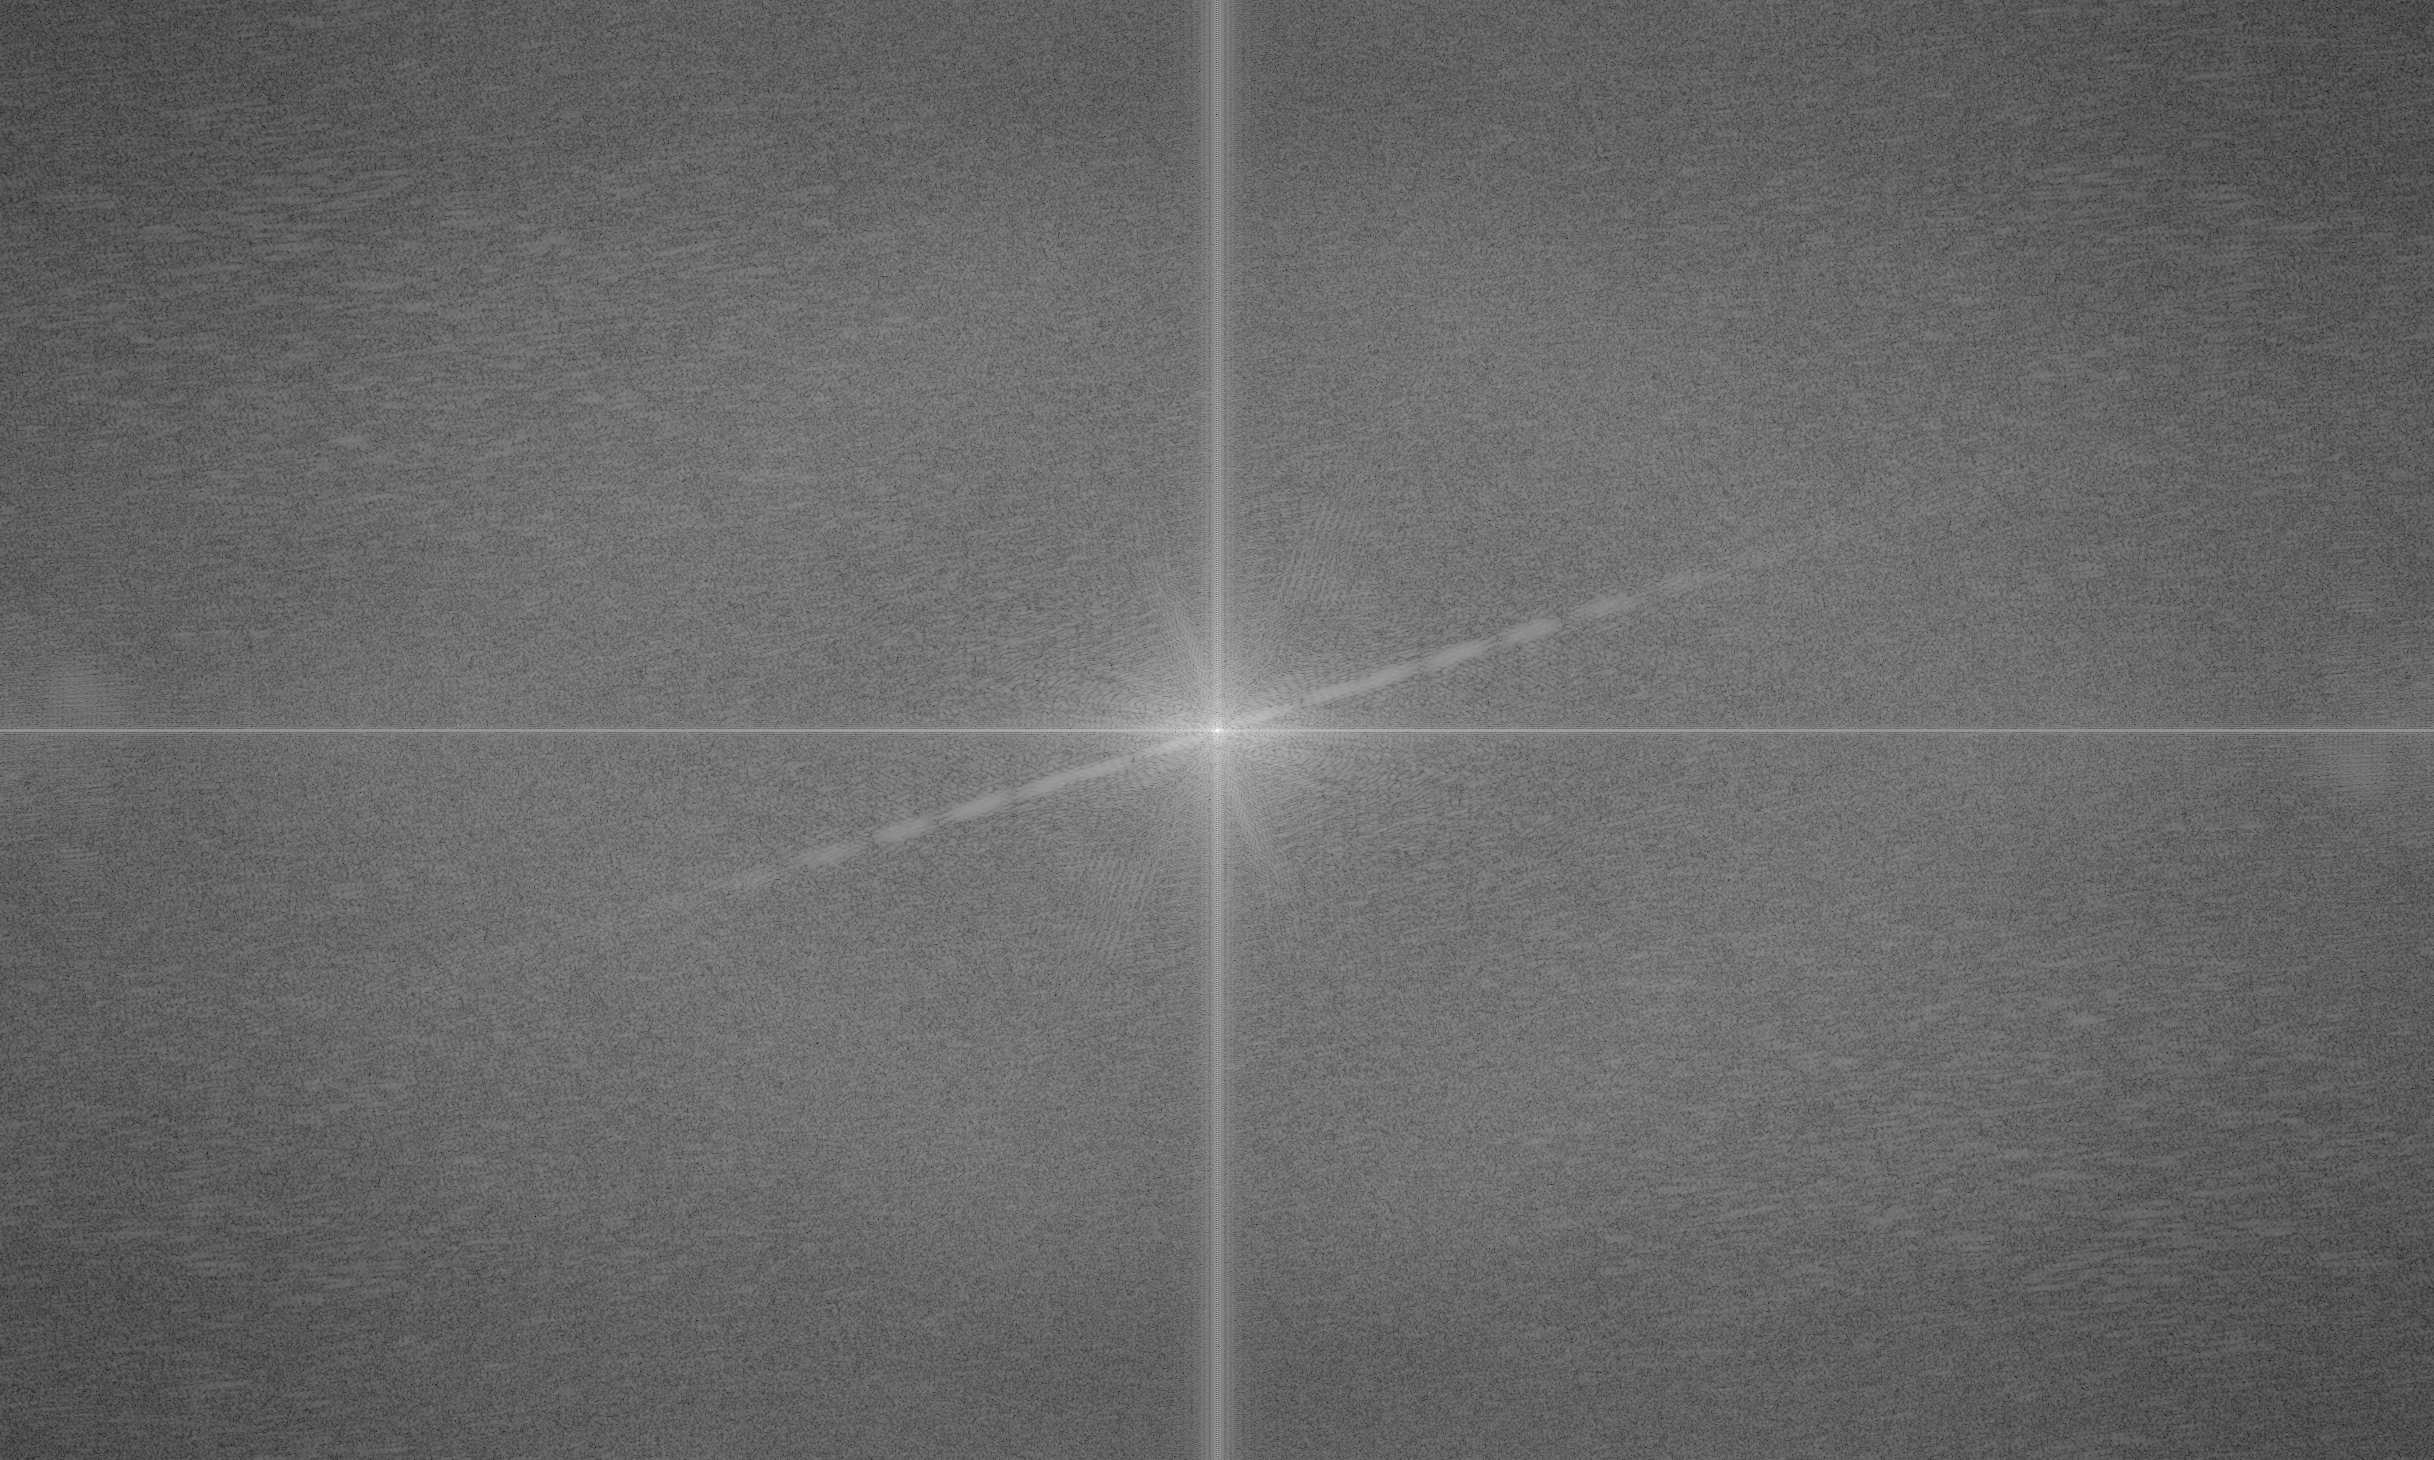
\includegraphics[width=0.47\textwidth]{sharpen_result_Gauss//sigma=20 c=1 filtered frequency.png}}
    \,    
    \subfigure[滤波效果]
    {\label{} 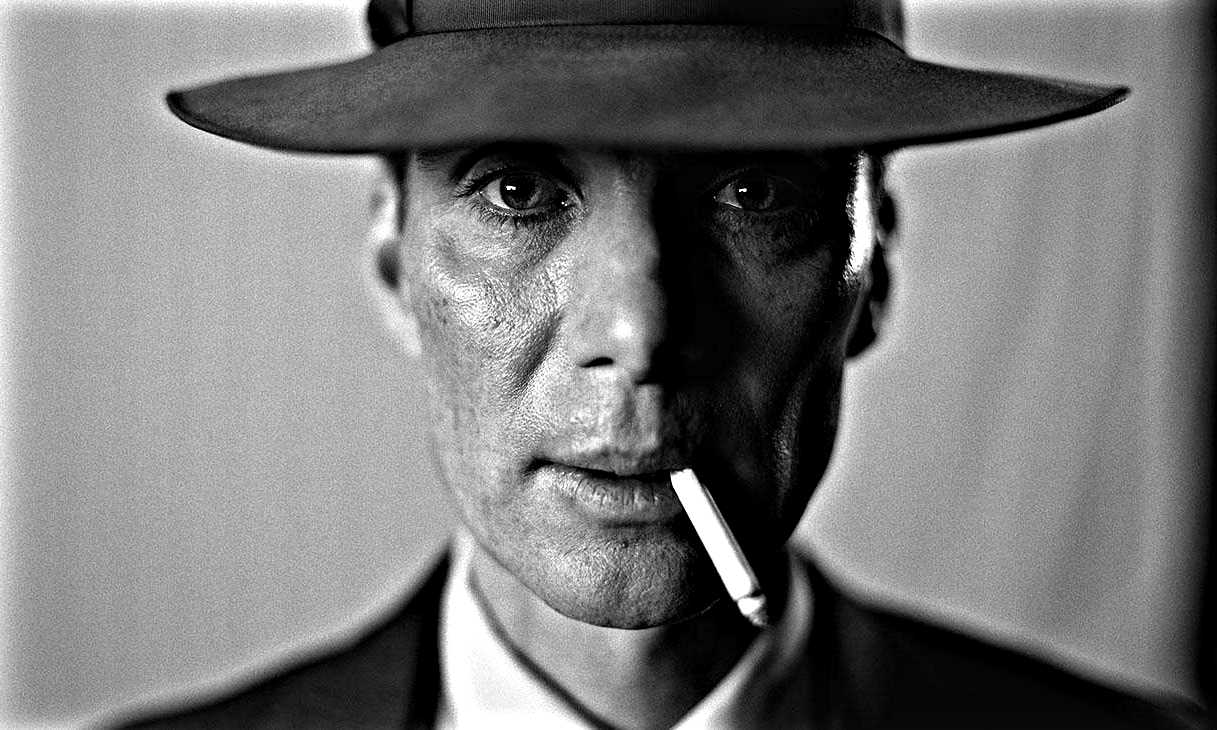
\includegraphics[width=0.47\textwidth]{sharpen_result_Gauss//sigma=20 c=1 filtered figure.png}}
    \caption{$\sigma=20$的频域高通滤波结果与效果图}\label{} 
\end{figure}


% \paragraph{$\sigma=40$的频域高通滤波结果与效果图}
\begin{figure}[H]
    \centering
    \subfigure[频域高通滤波结果(取对数)]
    {\label{} 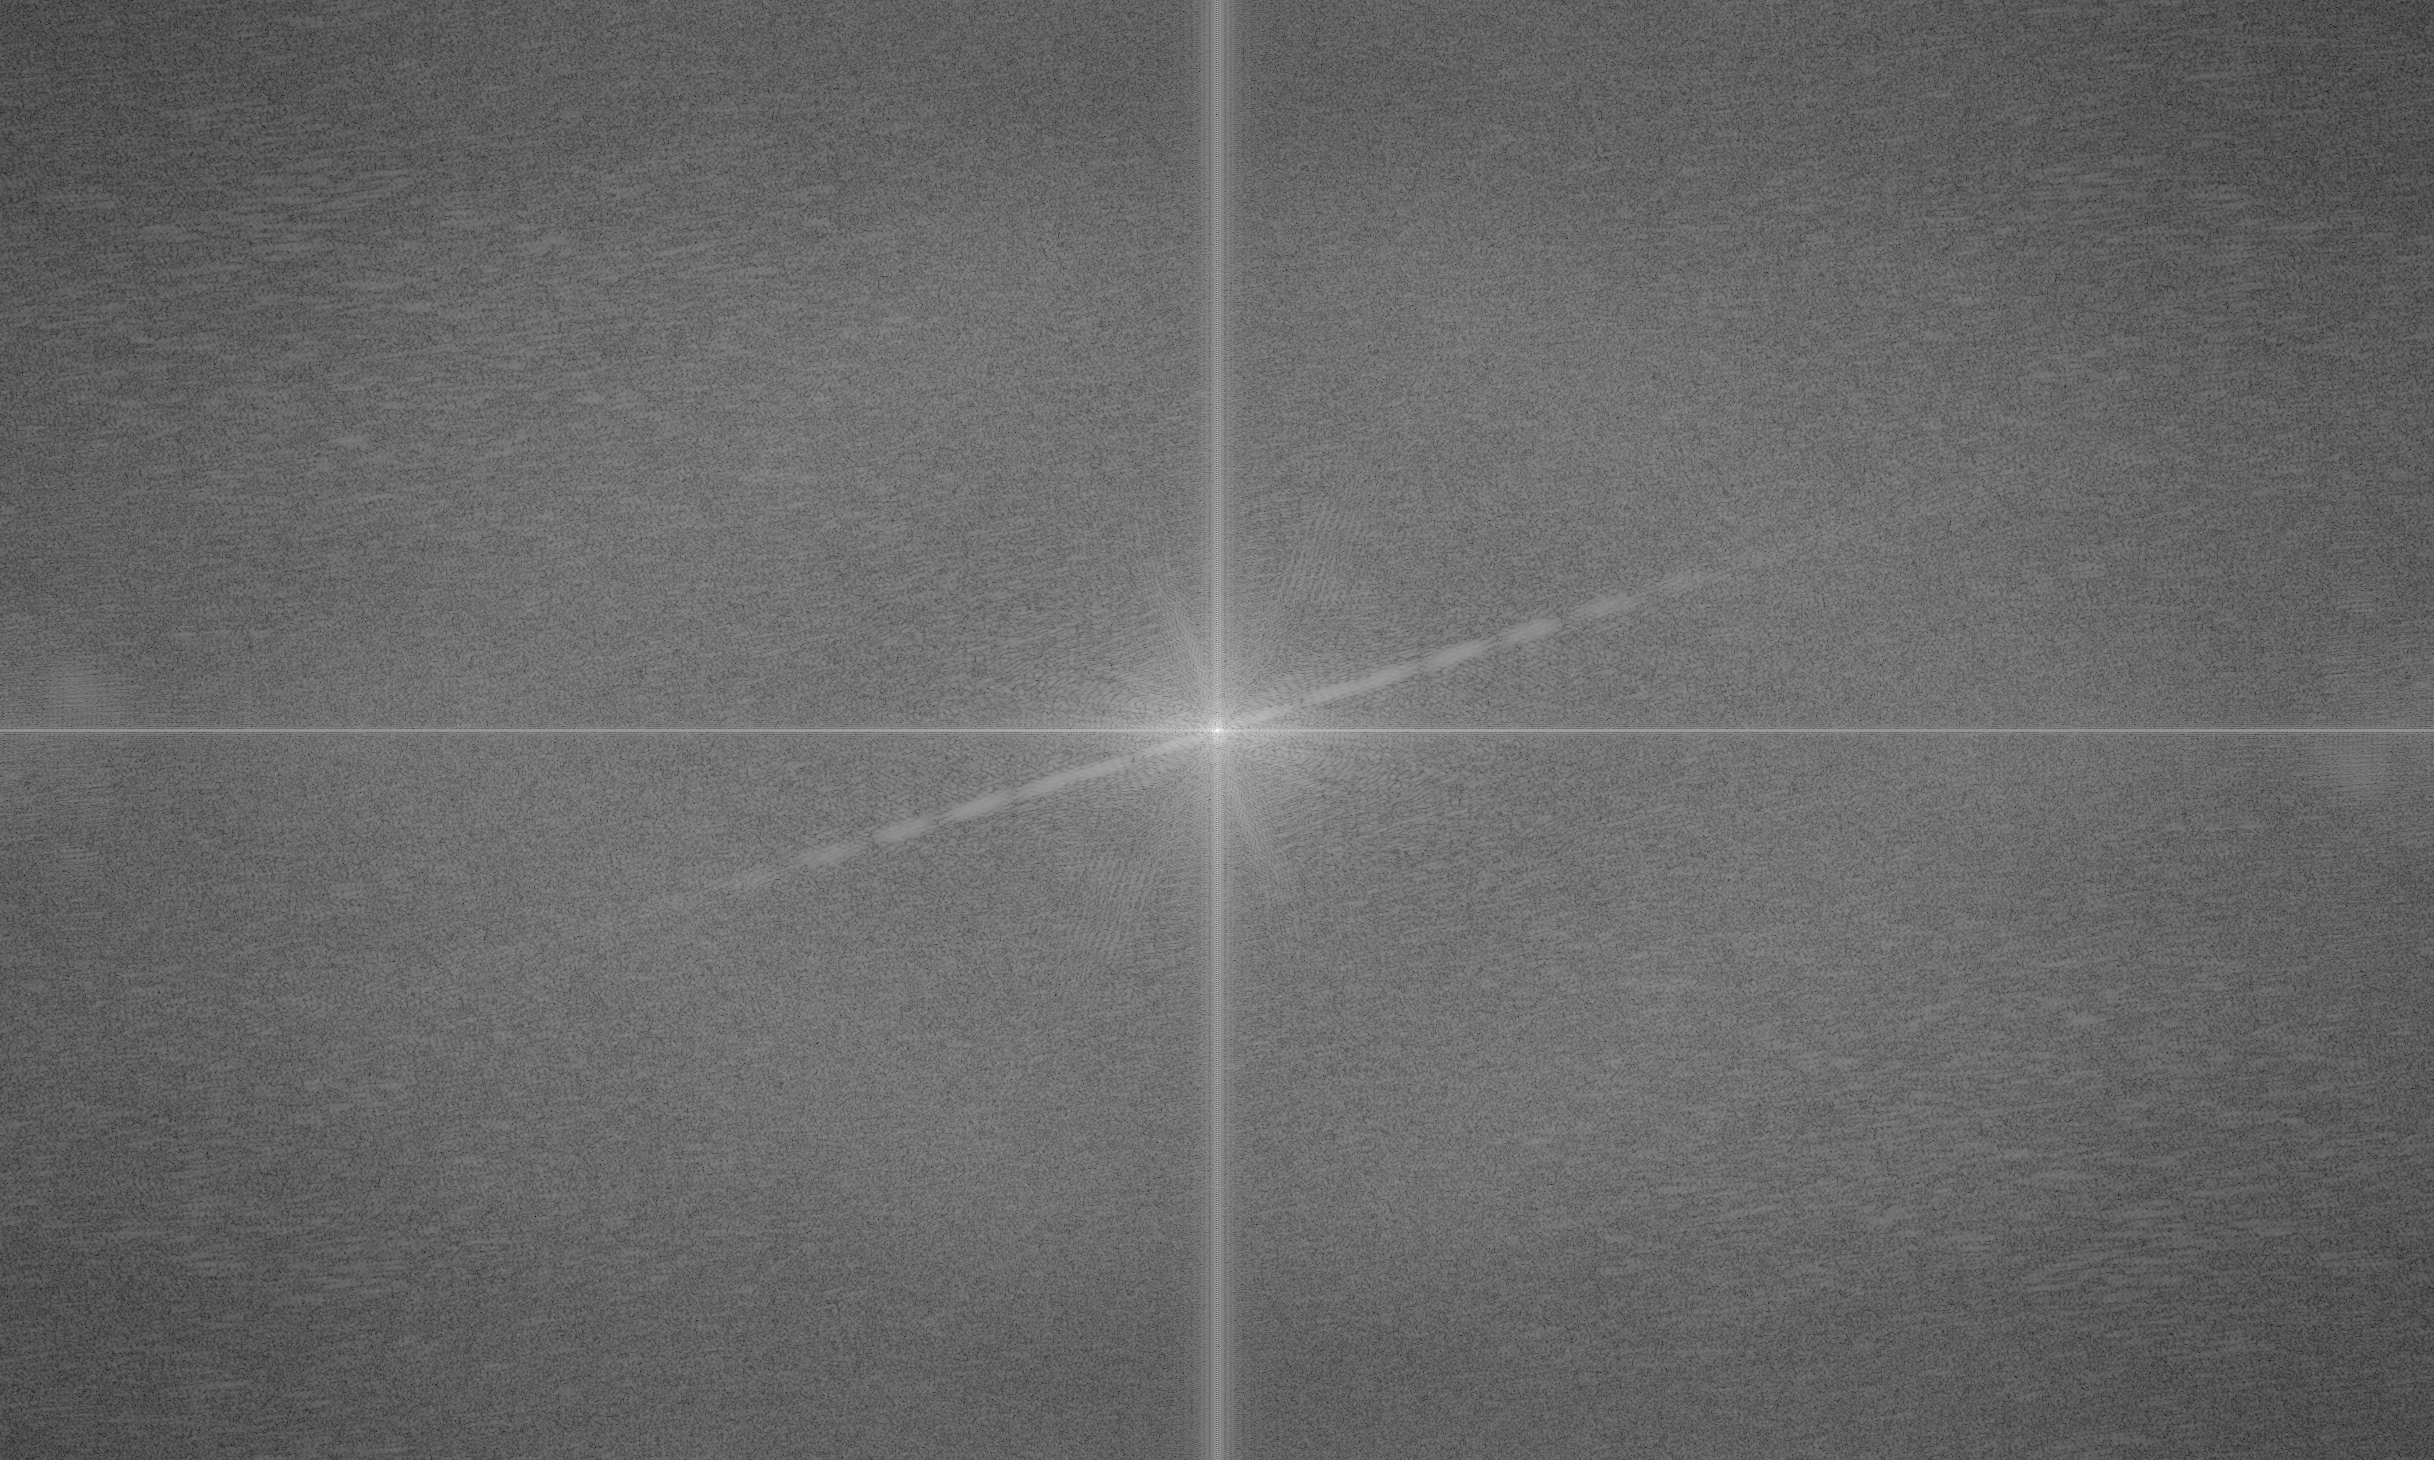
\includegraphics[width=0.47\textwidth]{sharpen_result_Gauss//sigma=40 c=1 filtered frequency.png}}
    \,    
    \subfigure[滤波效果]
    {\label{} 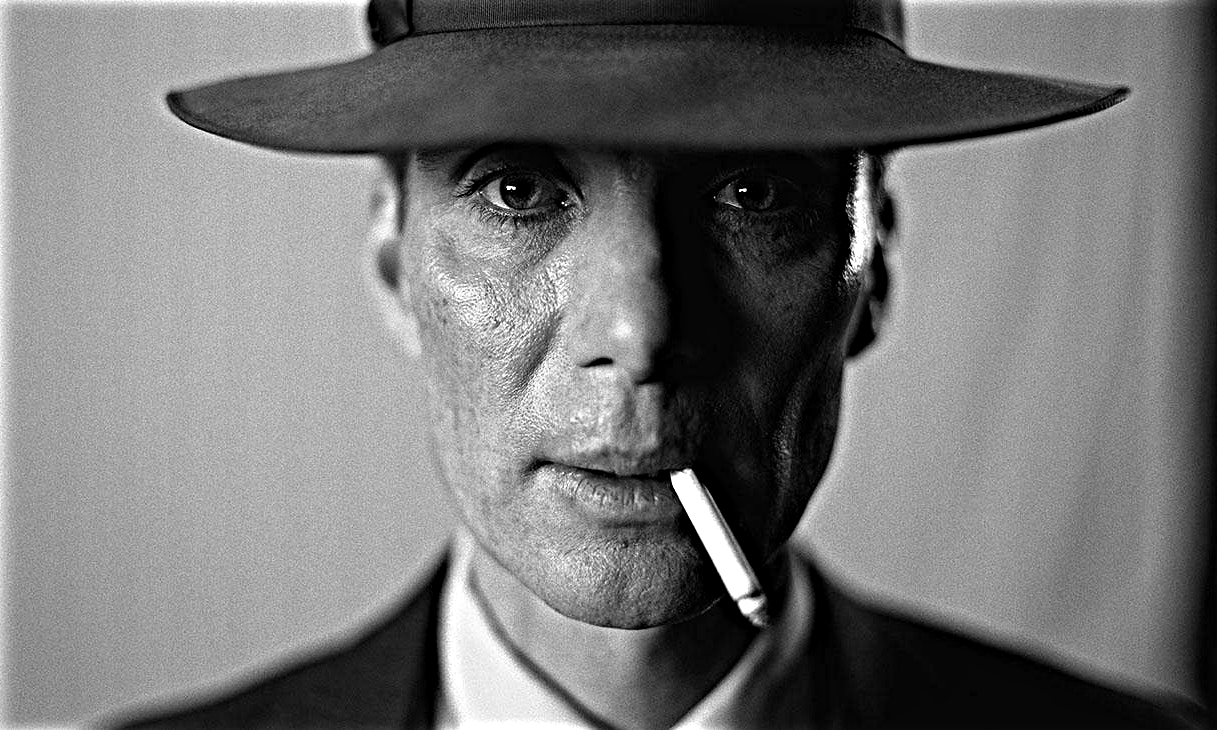
\includegraphics[width=0.47\textwidth]{sharpen_result_Gauss//sigma=40 c=1 filtered figure.png}}
    \caption{$\sigma=40$的频域高通滤波结果与效果图}\label{} 
\end{figure}

\paragraph{小结}
可以看出,\textbf{随着$\sigma$的增大,锐化的效果会越来越好},越来越多的细节会被展现出来,
但同时,当$\sigma>10$之后,锐化增强的程度逐渐下降,边际效应显著,这是因为频域中的
高频信号区域强度弱,而低频信号(频谱中心附近)区域的强度很强;当增大$\sigma$的时候,
虽然能过滤掉更大区域内的低频信号,但是当过滤区域从低频区扩展到高频区时,由于高频区域强度小,
则此时过滤和不过滤高频区的效果差异已经并不显著。

\section{去除大脑CT体膜图像中的条纹}

\subsection{频域变换}
体膜图的频域变换结果如下图\ref{CT}所示
\begin{figure}[H]
	\centering
	{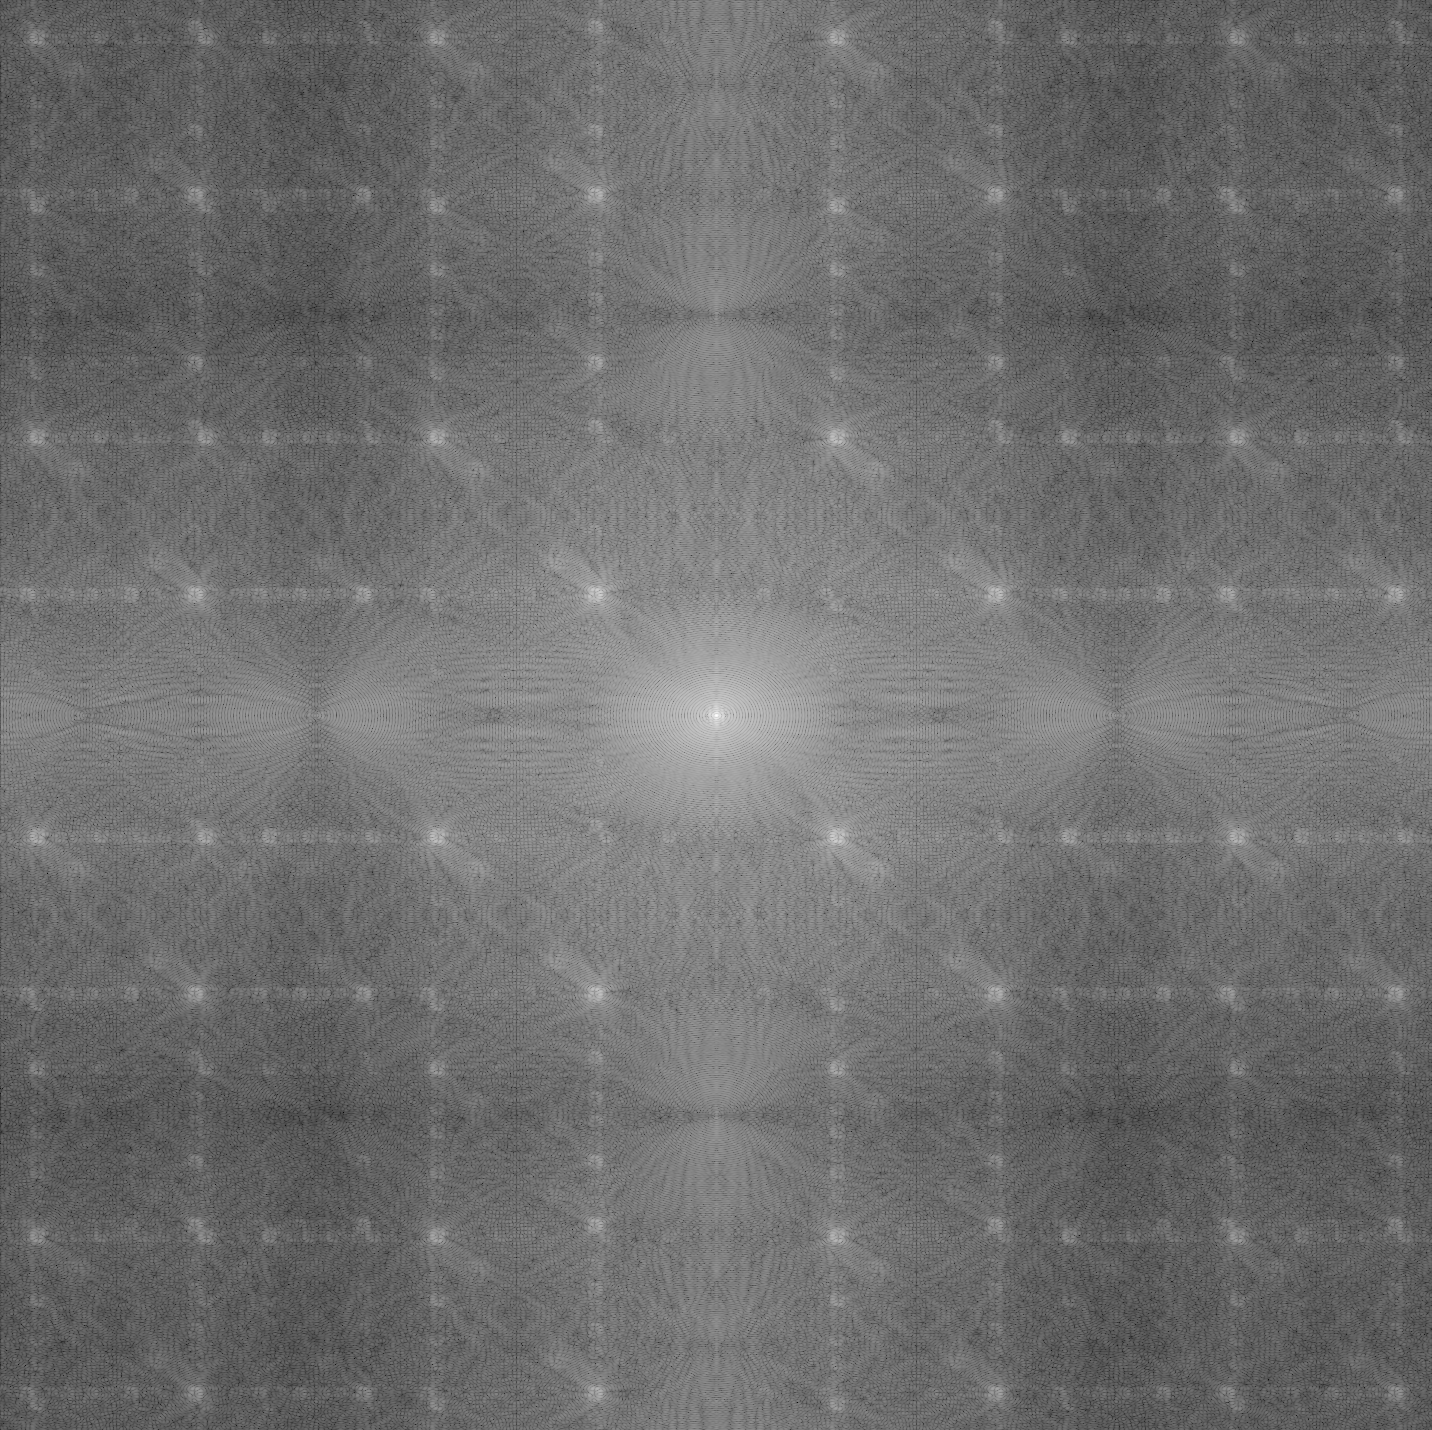
\includegraphics[width=0.5\textwidth]{remove_noise_result//frequency.png}} 
	\caption{大脑CT体膜图像的频域变换结果} \label{CT}
\end{figure}

注意到在频域的四个象限中,均有对称的网格状噪点,对应着原图的周期性噪音。我考虑的方案时:
仅保留中央的十字区域信号,而将四个象限中存在噪点的区域的信号全部舍弃。又考虑到如果直接用
box类函数会出现振铃效应(ringing effect),因此考虑使用高斯类的带通滤波器进行滤波。

我设计的频域带通滤波器如下:

\[
H(u,v) = \exp[-(u-u_0)^2/2\sigma_1^2] + \exp[-(v-v_0)^2/2\sigma_2^2]	
\]
其中$(u_0,v_0)$表示频域图像的中心。

经过尝试,我发现取$\sigma_1 =28,\, \sigma_2 = 28$会有比较良好的滤波效果,效果如图\ref{noise.main}所示。

\begin{figure}[H]
    \centering
    \subfigure[带通滤波结果(取对数)]
    {\label{noise.sub.1} 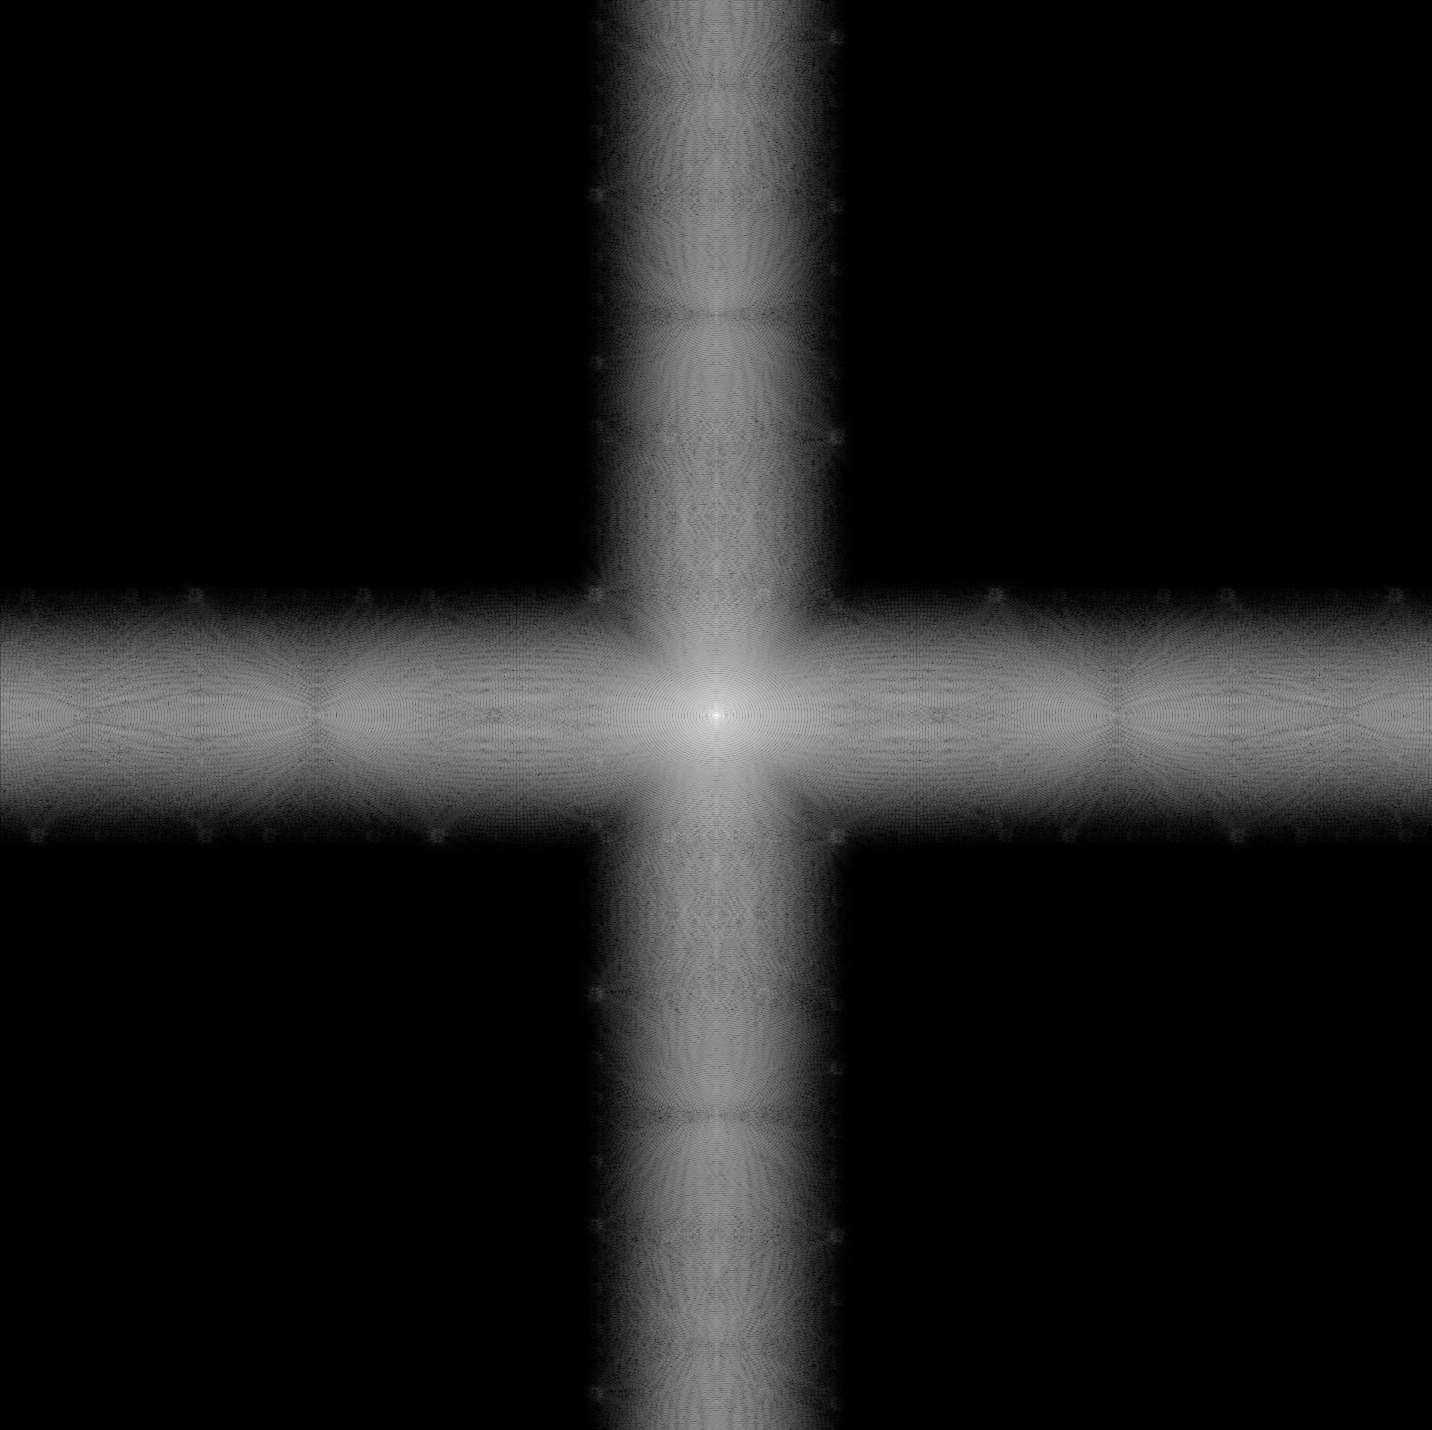
\includegraphics[width=0.47\textwidth]{remove_noise_result//filtered frequency.png}}
    \,    
    \subfigure[滤波效果]
    {\label{noise.sub.2} 
\includegraphics[width=0.47\textwidth]{remove_noise_result//result.png}}
    \caption{频域带通滤波结果与效果图}\label{noise.main} 
\end{figure}

\subsection{Python代码实现}
\lstinputlisting[style = Python,
caption={Python codes for removing noise},
label = {noise}]{2_remove_noise.py}


\end{document}

% \begin{figure}[H]
% 	\centering
% 	{\includegraphics[width=0.35\textwidth]{image//ignorance.png}} 
% 	\caption{} \label{} 
% \end{figure}


% \lstinputlisting[style = Python,
% caption={Python codes},
% label = {efficient},
% linerange={110-125}]{exercise3.py} 


% \begin{figure}[H]
%     \centering
%     \subfigure[patch size = 11]
%     {\label{} 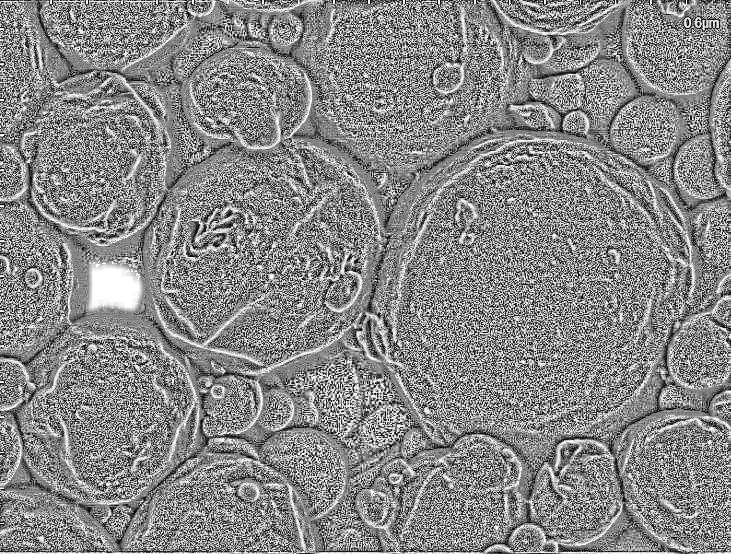
\includegraphics[width=0.47\textwidth]{image//local equalization with patch size = 11.jpg}}
%     \,    
%     \subfigure[patch size = 51]
%     {\label{} 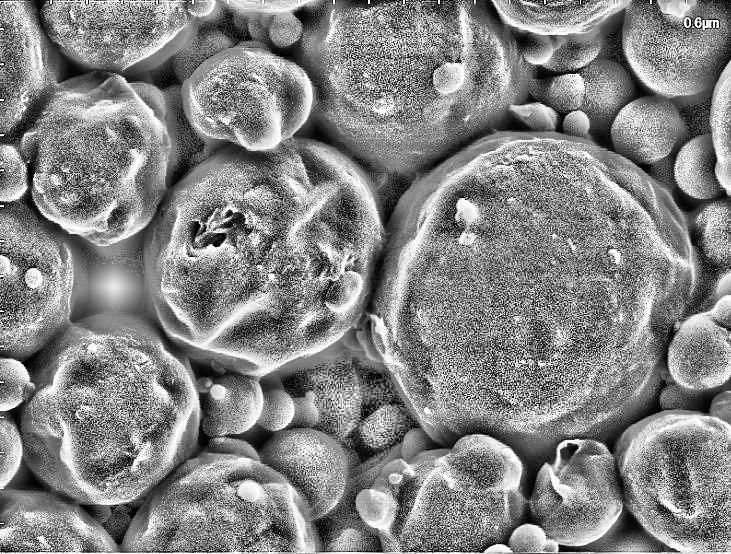
\includegraphics[width=0.47\textwidth]{image//local equalization with patch size = 51.jpg}}
%     \,
%     \subfigure[patch size = 151]
%     {\label{} 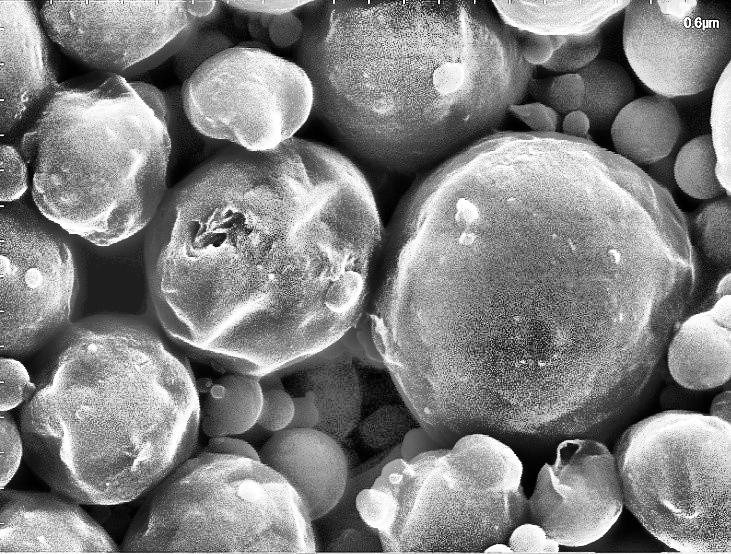
\includegraphics[width=0.47\textwidth]{image//local equalization with patch size = 151.jpg}}
%     \,    
%     \subfigure[patch size = 201]
%     {\label{} 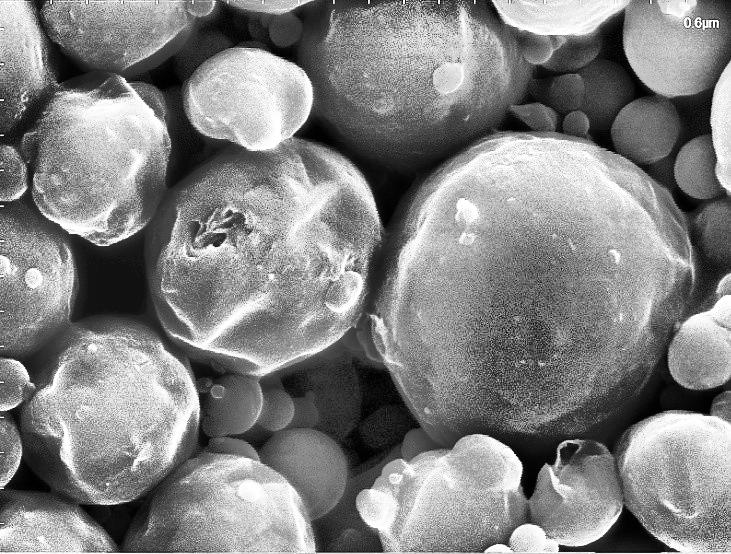
\includegraphics[width=0.47\textwidth]{image//local equalization with patch size = 201.jpg}}
%     \caption{local equalization with different patch sizes}\label{} 
% \end{figure}
